\documentclass[letterpaper, 12pt]{article}


\usepackage{/Users/zhengz/Desktop/Math/Workspace/Homework1/homework}
%%%%%%%%%%%%%%%%%%%%%%%%%%%%%%%%%%%%%%%%%%%%%%%%%%%%%%%%%%%%%%%%%%%%%%%%%%%%%%%%%%%%%%%%%%%%%%%%%%%%%%%%%%%%%%%%%%%%%%%%%%%%%%%%%%%%%%%%
\begin{document}
%Header-Make sure you update this information!!!!
\noindent
%%%%%%%%%%%%%%%%%%%%%%%%%%%%%%%%%%%%%%%%%%%%%%%%%%%%%%%%%%%%%%%%%%%%%%%%%%%%%%%%%%%%%%%%%%%%%%%%%%%%%%%%%%%%%%%%%%%%%%%%%%%%%%%%%%%%%%%%
\large\textbf{Zhengdong Zhang} \hfill \textbf{Homework 8}   \\
Email: zhengz@uoregon.edu \hfill ID: 952091294 \\
\normalsize Course: MATH 635 - Algebraic Topology II \hfill Term: Winter 2025\\
Instructor: Dr.Daniel Dugger \hfill Due Date: $7^{th}$ March, 2025 \\
\noindent\rule{7in}{2.8pt}
\setstretch{1.1}

%%%%%%%%%%%%%%%%%%%%%%%%%%%%%%%%%%%%%%%%%%%%%%%%%%%%%%%%%%%%%%%%%%%%%%%%%%%%%%%%%%%%%%%%%%%%%%%%%%%%%%%%%%%%%%%%%%%%%%%%%%%%%%%%%%%%%%%%
%Probelm 1 Connected
%%%%%%%%%%%%%%%%%%%%%%%%%%%%%%%%%%%%%%%%%%%%%%%%%%%%%%%%%%%%%%%%%%%%%%%%%%%%%%%%%%%%%%%%%%%%%%%%%%%%%%%%%%%%%%%%%%%%%%%%%%%%%%%%%%%%%%%%
\begin{problem}{1}
\begin{enumerate}[(a)]
\item If \(Z\) is \((n-1)\)-connected and \((X,A)\) is a relative CW-Complex of dimension \(\leq n\), prove that every solid-arrow diagram 
% https://q.uiver.app/#q=WzAsMyxbMCwwLCJBIl0sWzAsMSwiWCJdLFsxLDAsIloiXSxbMCwxLCIiLDAseyJzdHlsZSI6eyJ0YWlsIjp7Im5hbWUiOiJtb25vIn19fV0sWzAsMl0sWzEsMiwiIiwwLHsic3R5bGUiOnsiYm9keSI6eyJuYW1lIjoiZGFzaGVkIn19fV1d
\[\begin{tikzcd}
	A & Z \\
	X
	\arrow[from=1-1, to=1-2]
	\arrow[tail, from=1-1, to=2-1]
	\arrow[dashed, from=2-1, to=1-2]
\end{tikzcd}\]
has a lifting as shown. Include the case \(n=\infty\). 
\item Suppose \(Z\) is a CW complex that is \(k\)-connected, and let \(Z_k\) denote the \(k\)-skeleton. Prove that the inclusion \(Z_k\hookrightarrow Z\) extends over the cone on \(Z_k\), i.e. there is a lifting 
% https://q.uiver.app/#q=WzAsMyxbMCwwLCJaX2siXSxbMCwxLCJDKFpfaykiXSxbMSwwLCJaIl0sWzAsMSwiIiwwLHsic3R5bGUiOnsidGFpbCI6eyJuYW1lIjoibW9ubyJ9fX1dLFswLDIsIiIsMix7InN0eWxlIjp7InRhaWwiOnsibmFtZSI6Im1vbm8ifX19XSxbMSwyLCIiLDAseyJzdHlsZSI6eyJib2R5Ijp7Im5hbWUiOiJkYXNoZWQifX19XV0=
\[\begin{tikzcd}
	{Z_k} & Z \\
	{C(Z_k)}
	\arrow[tail, from=1-1, to=1-2]
	\arrow[tail, from=1-1, to=2-1]
	\arrow[dashed, from=2-1, to=1-2]
\end{tikzcd}\]
Then prove that the map \(Z\rightarrow Z/Z_k\) is a homotopy equivalence. 
\item Let \(Z\) be a CW complex that \(\pi_k(Z)=0\) for all \(k\geq 0\) (so \(Z\) is \(\infty\)-connected). Prove that \(Z\) is contractible.
\end{enumerate}
\end{problem}
\begin{solution}
\begin{enumerate}[(a)]
\item First we assume \(X\) is obtained from \(A\) by adding one \(k\)-cell (\(k\leq n\)). Given a map \(f:A\rightarrow Z\), we need to find a map \(\ti{f}:X\rightarrow Z\) such that \(\ti{f}i=f\) where 
\(i:A\rightarrow X\) is the inclusion map. Consider the pushout square from the cell structrue on the pair \((X,A)\) 
% https://q.uiver.app/#q=WzAsNCxbMSwwLCJBIl0sWzEsMSwiWCJdLFswLDAsIlNee2stMX0iXSxbMCwxLCJEXmsiXSxbMiwzXSxbMiwwXSxbMywxXSxbMCwxXV0=
\[\begin{tikzcd}
	{S^{k-1}} & A \\
	{D^k} & X
	\arrow["g",from=1-1, to=1-2]
	\arrow[from=1-1, to=2-1]
	\arrow["i", from=1-2, to=2-2]
	\arrow[from=2-1, to=2-2]
\end{tikzcd}\]
Consider the following solid-arrow diagram 
% https://q.uiver.app/#q=WzAsNSxbMSwwLCJBIl0sWzEsMSwiWCJdLFswLDAsIlNee2stMX0iXSxbMCwxLCJEXmsiXSxbMiwyLCJaIl0sWzIsM10sWzIsMCwiZyJdLFszLDFdLFswLDEsImkiLDJdLFswLDQsImYiLDAseyJjdXJ2ZSI6LTN9XSxbMyw0LCIiLDIseyJjdXJ2ZSI6M31dLFsxLDQsIlxcdGlsZGV7Zn0iLDIseyJzdHlsZSI6eyJib2R5Ijp7Im5hbWUiOiJkYXNoZWQifX19XV0=
\[\begin{tikzcd}
	{S^{k-1}} & A \\
	{D^k} & X \\
	&& Z
	\arrow["g", from=1-1, to=1-2]
	\arrow[from=1-1, to=2-1]
	\arrow["i"', from=1-2, to=2-2]
	\arrow["f", curve={height=-18pt}, from=1-2, to=3-3]
	\arrow[from=2-1, to=2-2]
	\arrow[curve={height=18pt}, from=2-1, to=3-3]
	\arrow["{\tilde{f}}"', dashed, from=2-2, to=3-3]
\end{tikzcd}\]
The outer square commutes because \(Z\) is \((n-1)\)-connected, so \(\pi_{k-1}(Z)=0\). This means the map \(fg:S^{k-1}\rightarrow Z\) is nullhomotopic, therefore we can extend \(gf\) to a map \(D^{k}\cong C(S^{k-1})\rightarrow Z\). By the universal property of pushout square, we 
have a map \(\ti{f}:X\rightarrow Z\) such that \(\ti{f}i=f\). 

Next we view \(Z\) as the empty map, and the above proof shows that \(i:A\rightarrow X\) has the LLP (left lifting property) with respect to \(Z\), if \(X\) is obtained from \(A\) by adding one \(k\)-cell. Now drop this assumption. Start with \(A\), we can build a CW structure by adding one \(k\)-cell at a time (\(k\leq n\)): 
\[A=X_0\hookrightarrow X_1\hookrightarrow X_2\hookrightarrow \cdots\]
where \(X=\colim_n X_n\). We have proved each \(X_i\rightarrow X_{i+1}\) has the LLP with respect to \(Z\). Applying what we proved in Problem 1, HW\#7, We know \(i:A\rightarrow X\) also has the LLP with respect to \(Z\). The case \(n=\infty\) is also included here because in this case, all homotopy groups of \(Z\) vanishes, so we can apply this method 
to all relative CW complex \((X,A)\) without restricting the dimension. 
\item To prove there exists such a lifting, it is the same as proving the inclusion map \(i_k:Z_k\hookrightarrow Z\) is nullhomotopic. We prove this by induction on \(k\). When \(k=0\), \(Z\) is path-connected and the inclusion \(i_0:Z_0\rightarrow Z\) is nullhomotopic by applying a path homotopy from each point 
in \(Z_0\) to the base point. Now assume we have proved the case for \(k-1\) (\(k\geq 1\)), we are going to show that \(i_k:Z_k\rightarrow Z\) is nullhomotopic if \(Z\) is \(k\)-connected. We know that the map \(i_{k-1}:Z_{k-1}\rightarrow Z\) is nullhomotopic, so there exists a homotopy 
\(H_{k-1}:Z_{k-1}\times I\rightarrow Z\) such that \(H(-,0)=i_{k-1}\) and \(H(-,1)=*\) is constant. Note that \(H(-,0)=i_k|_{Z_{k-1}}\) and \((Z_k,Z_{k-1})\) is a CW pair, by HEP we have a lifting 
% https://q.uiver.app/#q=WzAsMyxbMCwwLCJaX2tcXHRpbWVzXFxsZWZ0XFx7MFxccmlnaHRcXH1cXGN1cCBaX3trLTF9XFx0aW1lcyBJIl0sWzAsMSwiWl9rXFx0aW1lcyBJIl0sWzIsMCwiWiJdLFswLDIsImlfa1xcY3VwIEhfe2stMX0iXSxbMCwxXSxbMSwyLCJIX2siLDIseyJzdHlsZSI6eyJib2R5Ijp7Im5hbWUiOiJkYXNoZWQifX19XV0=
\[\begin{tikzcd}
	{Z_k\times\left\{0\right\}\cup Z_{k-1}\times I} && Z \\
	{Z_k\times I}
	\arrow["{i_k\cup H_{k-1}}", from=1-1, to=1-3]
	\arrow[from=1-1, to=2-1]
	\arrow["{H_k}"', dashed, from=2-1, to=1-3]
\end{tikzcd}\]
\(H_k(-,1):Z_k\rightarrow Z\) is homotopic to \(i_k\) and it sends \(Z_{k-1}\subseteq Z_k\) to a point in \(Z\). So \(H(-,1)\) must factor through \(Z_k/Z_{k-1}\cong \vee_\alpha S^k\).
% https://q.uiver.app/#q=WzAsMyxbMCwwLCJaX2siXSxbMiwwLCJaIl0sWzAsMSwiWl9rL1pfe2stMX1cXGNvbmcgXFx2ZWUgU15rIl0sWzAsMSwiSCgtLDEpIl0sWzAsMiwicSIsMl0sWzIsMSwiaCIsMl1d
\[\begin{tikzcd}
	{Z_k} && Z \\
	{Z_k/Z_{k-1}\cong \vee S^k}
	\arrow["{H(-,1)}", from=1-1, to=1-3]
	\arrow["q"', from=1-1, to=2-1]
	\arrow["h"', from=2-1, to=1-3]
\end{tikzcd}\]
Note that \(Z\) is \(k\)-connected, so \(h:\vee S^k\rightarrow Z\) as a composition of elements in \(\pi_k(Z)\) is also nullhomotopic. By precompsoing with the quotient the map \(q\), we have proved \(H(-,1)\) is nullhomotopic. 

Now we need to show that the quotient map \(q_k:Z\rightarrow Z/Z_k\) is a homotopy equivalence. We have proved \(i_k:Z_k\rightarrow Z\) is nullhomotopic, so there exists a map \(J:Z_k\rightarrow Z\) such that \(J(-,0)=i_k\) and \(J(-,1)=*\) is constant. Note that 
\((Z,Z_k)\) is a CW pair and \(id_Z|_{Z_k}=i_k\), by HEP, we have 
% https://q.uiver.app/#q=WzAsMyxbMCwwLCJaXFx0aW1lcyBcXGxlZnRcXHswXFxyaWdodFxcfVxcY3VwIFpfa1xcdGltZXMgSSJdLFsyLDAsIloiXSxbMCwxLCJaXFx0aW1lcyBJIl0sWzAsMSwiaWRfWlxcY3VwIEoiXSxbMCwyXSxbMiwxLCJLIiwyLHsic3R5bGUiOnsiYm9keSI6eyJuYW1lIjoiZGFzaGVkIn19fV1d
\[\begin{tikzcd}
	{Z\times \left\{0\right\}\cup Z_k\times I} && Z \\
	{Z\times I}
	\arrow["{id_Z\cup J}", from=1-1, to=1-3]
	\arrow[from=1-1, to=2-1]
	\arrow["K"', dashed, from=2-1, to=1-3]
\end{tikzcd}\]
Here \(K(-,0)=id_Z\) and \(K(0,1):Z\rightarrow Z\) sends the \(k\)-skeleton \(Z_k\) to a point. So \(K(-,1)\) must factor through the quotient \(Z/Z_k\), and we have a map \(f:Z/Z_k\rightarrow Z\) such that \(fq_k=K(-,1)\).
% https://q.uiver.app/#q=WzAsMyxbMCwwLCJaIl0sWzEsMCwiWiJdLFswLDEsIlovWl9rIl0sWzAsMiwicV9rIiwyXSxbMiwxLCJmIiwyLHsic3R5bGUiOnsiYm9keSI6eyJuYW1lIjoiZGFzaGVkIn19fV0sWzAsMSwiSygtLDEpIl1d
\[\begin{tikzcd}
	Z & Z \\
	{Z/Z_k}
	\arrow["{K(-,1)}", from=1-1, to=1-2]
	\arrow["{q_k}"', from=1-1, to=2-1]
	\arrow["f"', dashed, from=2-1, to=1-2]
\end{tikzcd}\]
We have \(q_kf=id:Z/Z_k\rightarrow Z\rightarrow Z/Z_k\) because \(q_k\) sends all cells in \(Z_k\) to a point in \(Z\). On the other hand, by definition we have \(fq_k=K(-,1)\) is homotopic to the identity map \(K(-,0)=id_Z\). This proves that 
\(q_k:Z\rightarrow Z/Z_k\) is a homotopy equivalence. 
\item Let \(CZ\) be the cone over \(Z\), namely \(Z\times I/Z\times \left\{ 1 \right\}\). To show that \(Z\) is homotopy equivalent to a point, it is enough to show that the identity map \(id:Z\rightarrow Z\) is nullhomotopic. This implies the composition 
\(Z\rightarrow \left\{ * \right\}\rightarrow Z\) is homotopic to the identity map \(Z\rightarrow Z\). So we have the homotopy equivalence. From what we discuss in the last part, showing \(id:Z\rightarrow Z\) is nullhomotopic is the same as showing 
the solid-arrow diagram 
% https://q.uiver.app/#q=WzAsMyxbMCwwLCJaIl0sWzEsMCwiWiJdLFswLDEsIkNaIl0sWzAsMl0sWzAsMSwiaWQiXSxbMiwxLCIiLDIseyJzdHlsZSI6eyJib2R5Ijp7Im5hbWUiOiJkYXNoZWQifX19XV0=
\[\begin{tikzcd}
	Z & Z \\
	CZ
	\arrow["id", from=1-1, to=1-2]
	\arrow["i", from=1-1, to=2-1]
	\arrow[dashed, from=2-1, to=1-2]
\end{tikzcd}\]
has a lifting. We prove this by show that \((CZ,Z)\) has a relative CW structure. Let \(X_{-1}=Z\) and \(X_0=Z\cup \left\{ * \right\}\), where the 0-cell \(*\) corresponds to the point \(X\times \left\{ 1 \right\}\) in the cone. For any 
\(0\)-cell (point) \(z\in Z\), we add a \(1\)-cell \(\ell_z\), whose boundary is mapped to \(*\) and \(z\). The resulted CW complex is denoted by \(X_1\). Next, for any 1-cell \(\Delta_1\) in \(Z\), the boundary of \(\Delta_1\) must be two 0-cells (possibly the same). We add a \(2\)-cell whose boundary is mapped 
to the \(1\)-cells \(\ell_{z_1}\), \(\ell_{z_2}\) and \(\Delta_1\) (as shown in picture). The resulted CW complex is denoted by \(X_2\). 
\[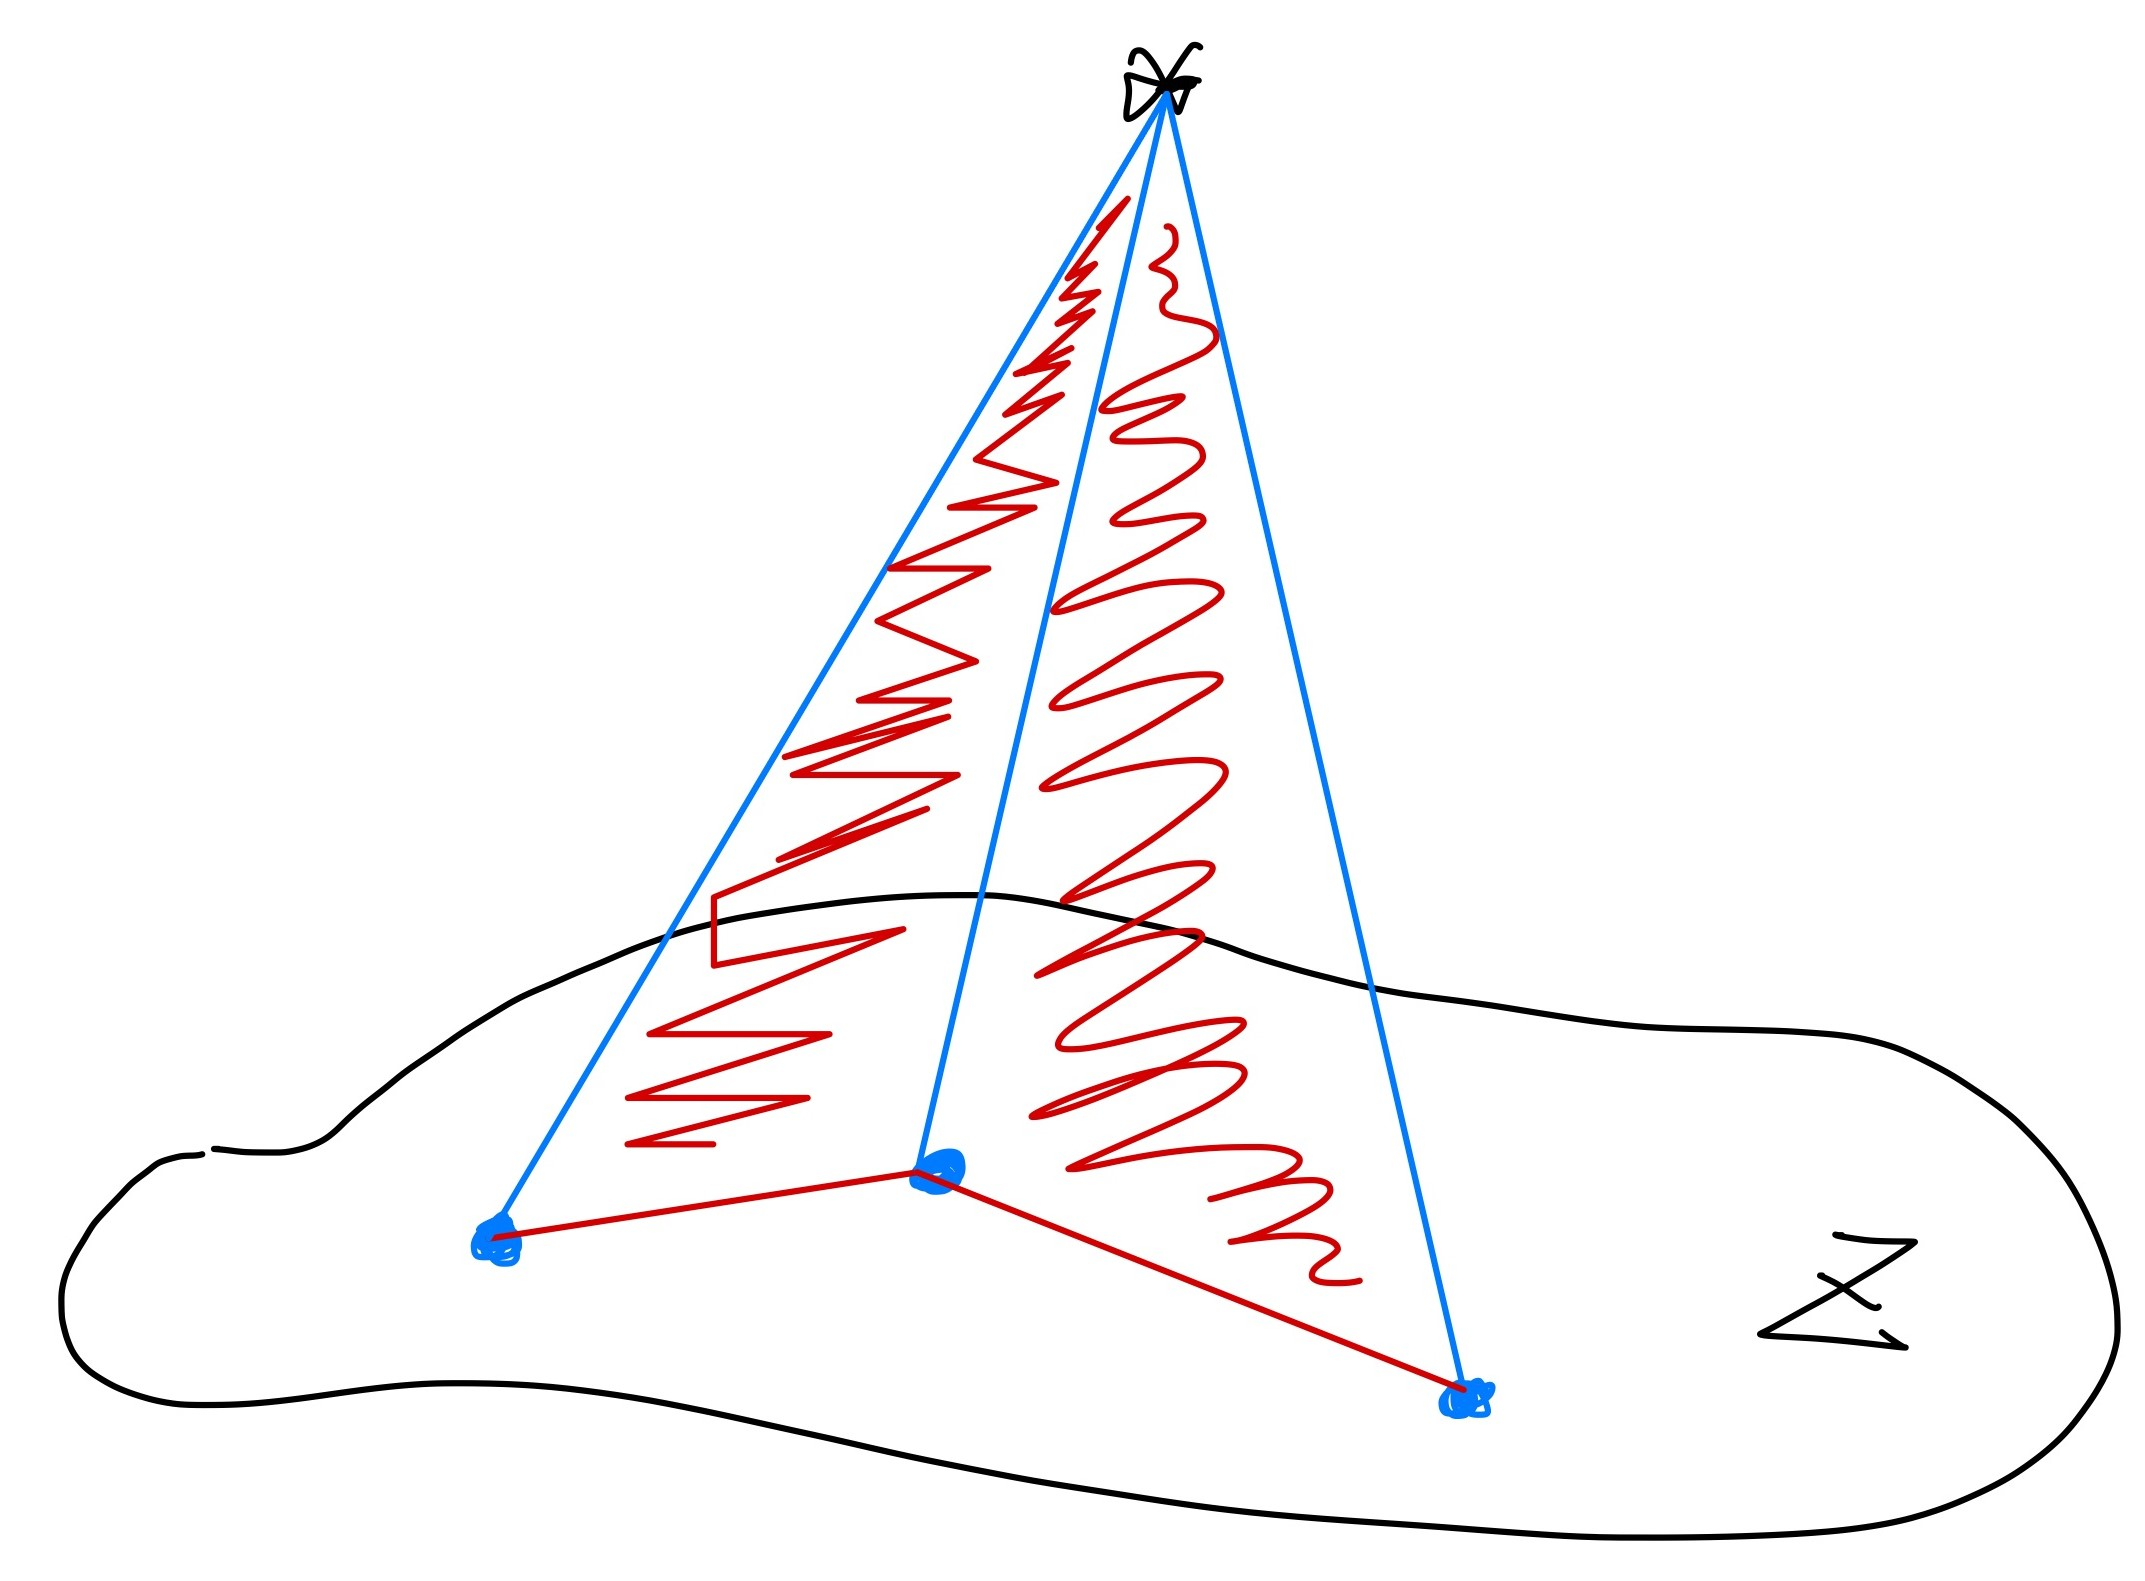
\includegraphics[scale=0.1]{Pictures/HW8-1-1.jpg}\]
We can do it inductively and obtain a sequence of CW complex 
\[Z=X_{-1}\hookrightarrow X_0\hookrightarrow X_1\hookrightarrow\cdots\]
By our construction, the colimit \(\colim_n X_n\) of this sequence is isomorphic to the cone over \(Z\). For any \(i\geq 0\), we know \(X_i\) is just adding cells of dimension \(\leq i\) to the previous space \(X_{i-1}\). From Homework \#7 problem 1, we know we have a lifting 
% https://q.uiver.app/#q=WzAsMyxbMCwwLCJaIl0sWzEsMCwiWiJdLFswLDEsIlhfaSJdLFswLDJdLFswLDEsImlkIl0sWzIsMSwiIiwyLHsic3R5bGUiOnsiYm9keSI6eyJuYW1lIjoiZGFzaGVkIn19fV1d
\[\begin{tikzcd}
	Z & Z \\
	{X_0}
	\arrow["id", from=1-1, to=1-2]
	\arrow[from=1-1, to=2-1]
	\arrow[dashed, from=2-1, to=1-2]
\end{tikzcd}\]
And the lifting exists if we do this inductively for each \(X_{i-1}\rightarrow X_i\). Then we know we also has a lifting for the colimit 
% https://q.uiver.app/#q=WzAsMyxbMCwwLCJaIl0sWzEsMCwiWiJdLFswLDEsIkNaIl0sWzAsMl0sWzAsMSwiaWQiXSxbMiwxLCIiLDIseyJzdHlsZSI6eyJib2R5Ijp7Im5hbWUiOiJkYXNoZWQifX19XV0=
\[\begin{tikzcd}
	Z & Z \\
	CZ
	\arrow["id", from=1-1, to=1-2]
	\arrow[from=1-1, to=2-1]
	\arrow[dashed, from=2-1, to=1-2]
\end{tikzcd}\] 
\end{enumerate}
\end{solution}

\noindent\rule{7in}{2.8pt}
%%%%%%%%%%%%%%%%%%%%%%%%%%%%%%%%%%%%%%%%%%%%%%%%%%%%%%%%%%%%%%%%%%%%%%%%%%%%%%%%%%%%%%%%%%%%%%%%%%%%%%%%%%%%%%%%%%%%%%%%%%%%%%%%%%%%%%%%
%Probelm 2
%%%%%%%%%%%%%%%%%%%%%%%%%%%%%%%%%%%%%%%%%%%%%%%%%%%%%%%%%%%%%%%%%%%%%%%%%%%%%%%%%%%%%%%%%%%%%%%%%%%%%%%%%%%%%%%%%%%%%%%%%%%%%%%%%%%%%%%%
\begin{problem}{2}
Let \(p:E\rightarrow B\) be a covering space, and let \(b\in B\). Without using any fancy theory, prove the following. If \(e,f\in p^{-1}(b)\) are in the same path component of \(E\), then 
\(p_*(\pi_1(E,e))\) and \(p_*(\pi_1(E,f))\) are conjugate subgroups of \(\pi_1(B,b)\).
\end{problem}
\begin{solution}
Let \(\gamma:I\rightarrow E\) be a path in \(E\) such that \(\gamma(0)=e\) and \(\gamma(1)=f\). For any element \([\lambda]\in \pi_1(E,f)\), where \(\lambda:I\rightarrow E\) is a loop based on \(f\) (\(\lambda(0)=\lambda(1)=f\)), we have an isomorphism of groups 
\(F:\pi_1(E,f)\xrightarrow{\sim}\pi_1(E,e)\) by sending \([\lambda]\) to \([\gamma^{-1}*\lambda*\gamma]\). By definiton, \(p_*:\pi_1(E,e)\rightarrow \pi_1(B,b)\) sends \([\gamma^{-1}*\lambda*\gamma]\) to \([p\circ(\gamma^{-1}* \lambda*\gamma)]\). 
\begin{claim}
For any two paths \(\alpha,\beta:I\rightarrow E\) satisfying \(\beta(0)=\alpha(1)\), we have 
\[p\circ (\beta*\alpha)=(p\circ \beta)*(p\circ \alpha).\]
\end{claim}
\begin{claimproof}
By definition 
\[(\beta*\alpha)(t)=\begin{cases}
	\alpha(2t),&\iif 0\leq t\leq \frac{1}{2},\\ 
	\beta(2t-1),&\iif \frac{1}{2}\leq t\leq 1.
\end{cases}\]
So we have 
\[(p\circ (\beta*\alpha))(t)=\begin{cases}
	(p\circ \alpha)(2t),&\iif 0\leq t\leq \frac{1}{2},\\ 
	(p\circ \beta)(2t-1),&\iif \frac{1}{2}\leq t\leq 1.
\end{cases}\]
This is exactly the definition of \((p\circ \beta)*(p\circ \alpha)\)
\end{claimproof}

For any \([\lambda]\in \pi_1(E,f)\), the image 
\begin{align*}
(p_*\circ F)([\lambda])&=p_*([\gamma^{-1}*\lambda*\gamma])\\ 
                       &=[p\circ (\gamma^{-1}*\lambda*\gamma)]\\ 
					   &=[(p\circ \gamma^{-1})*(p\circ \lambda)*(p\circ \gamma)].
\end{align*}
Note that \((p\circ \gamma)(0)=p(e)=p(f)=(p\circ \gamma)(1)\). So \([p\circ \gamma^{-1}]\) and \([p\circ \gamma]\) are loops based at \(b\) in \(B\). Moreover, note that 
\[[(p\circ \gamma^{-1})*(p\circ \gamma)]=[p\circ (\gamma^{-1}*\gamma)]=[p\circ C_e]=[C_b]\]
is the identity element in \(\pi_1(B,b)\), so they are inverse to each other. The group operation in \(\pi_1(B,b)\) is given by concatenation and note that \([p\circ \lambda]\in p_*(\pi_1(E,f))\). This proves that every element 
in \(p_*(\pi_1(E,e))\) can be written as a conjugate of an element in \(p_*(\pi_1(E,f))\). So \(p_*(\pi_1(E,e))\) and \(p_*(\pi_1(E,f))\) are conjugate subgroups of \(\pi_1(B,b)\). 
\end{solution}

\noindent\rule{7in}{2.8pt}
%%%%%%%%%%%%%%%%%%%%%%%%%%%%%%%%%%%%%%%%%%%%%%%%%%%%%%%%%%%%%%%%%%%%%%%%%%%%%%%%%%%%%%%%%%%%%%%%%%%%%%%%%%%%%%%%%%%%%%%%%%%%%%%%%%%%%%%%
%Probelm 3
%%%%%%%%%%%%%%%%%%%%%%%%%%%%%%%%%%%%%%%%%%%%%%%%%%%%%%%%%%%%%%%%%%%%%%%%%%%%%%%%%%%%%%%%%%%%%%%%%%%%%%%%%%%%%%%%%%%%%%%%%%%%%%%%%%%%%%%%
\begin{problem}{3}
\begin{enumerate}[(a)]
\item You know the universal covering spaces of \(\mathbb{R}P^2\) and \(S^1\). Using this knowledge (and thinking about the example of \(S_1\vee S_1\)) draw a picture of the universal covering spaces of 
\(S_2\vee S_1\), \(\mathbb{R}P^2\vee \mathbb{R}P^2\), \(\mathbb{R}P^2\vee S^2\) and \(\mathbb{R}P^2\vee S_1\). 
\item Determine how many 3-fold path-connected covering spaces of \(\mathbb{R}P^2\vee \mathbb{R}P^2\) there are, and draw pictures.
\end{enumerate}
\end{problem}
\begin{solution}
\begin{enumerate}[(a)]
\item We describe a general way to construct the universal coverings for the wedge sum \(X\vee Y\). Let \(\ti{X}\) and \(\ti{Y}\) be the universal covering of \(X\) and \(Y\) respectively. To construct the universal covering for 
\(X\vee Y\), first we take \(\ti{X}\), find all the preimages of the wedge points in \(\ti{X}\), and glue a copy of \(\ti{Y}\) along each preimage. Next, we look at the preimage of the wedge point in \(\ti{Y}\)'s we glued, and glue a 
copy of \(\ti{X}\) along each preimage if no \(\ti{X}\) is attached to that point. Note that every time no intersection happens for two different gluing process. We can do it continously and take the colimit. The resulting space is the universal covering 
for \(X\vee Y\). We include the universal coverings for different spaces in the following pictures. This is the universal covering of \(S^2\vee S^1\).
\[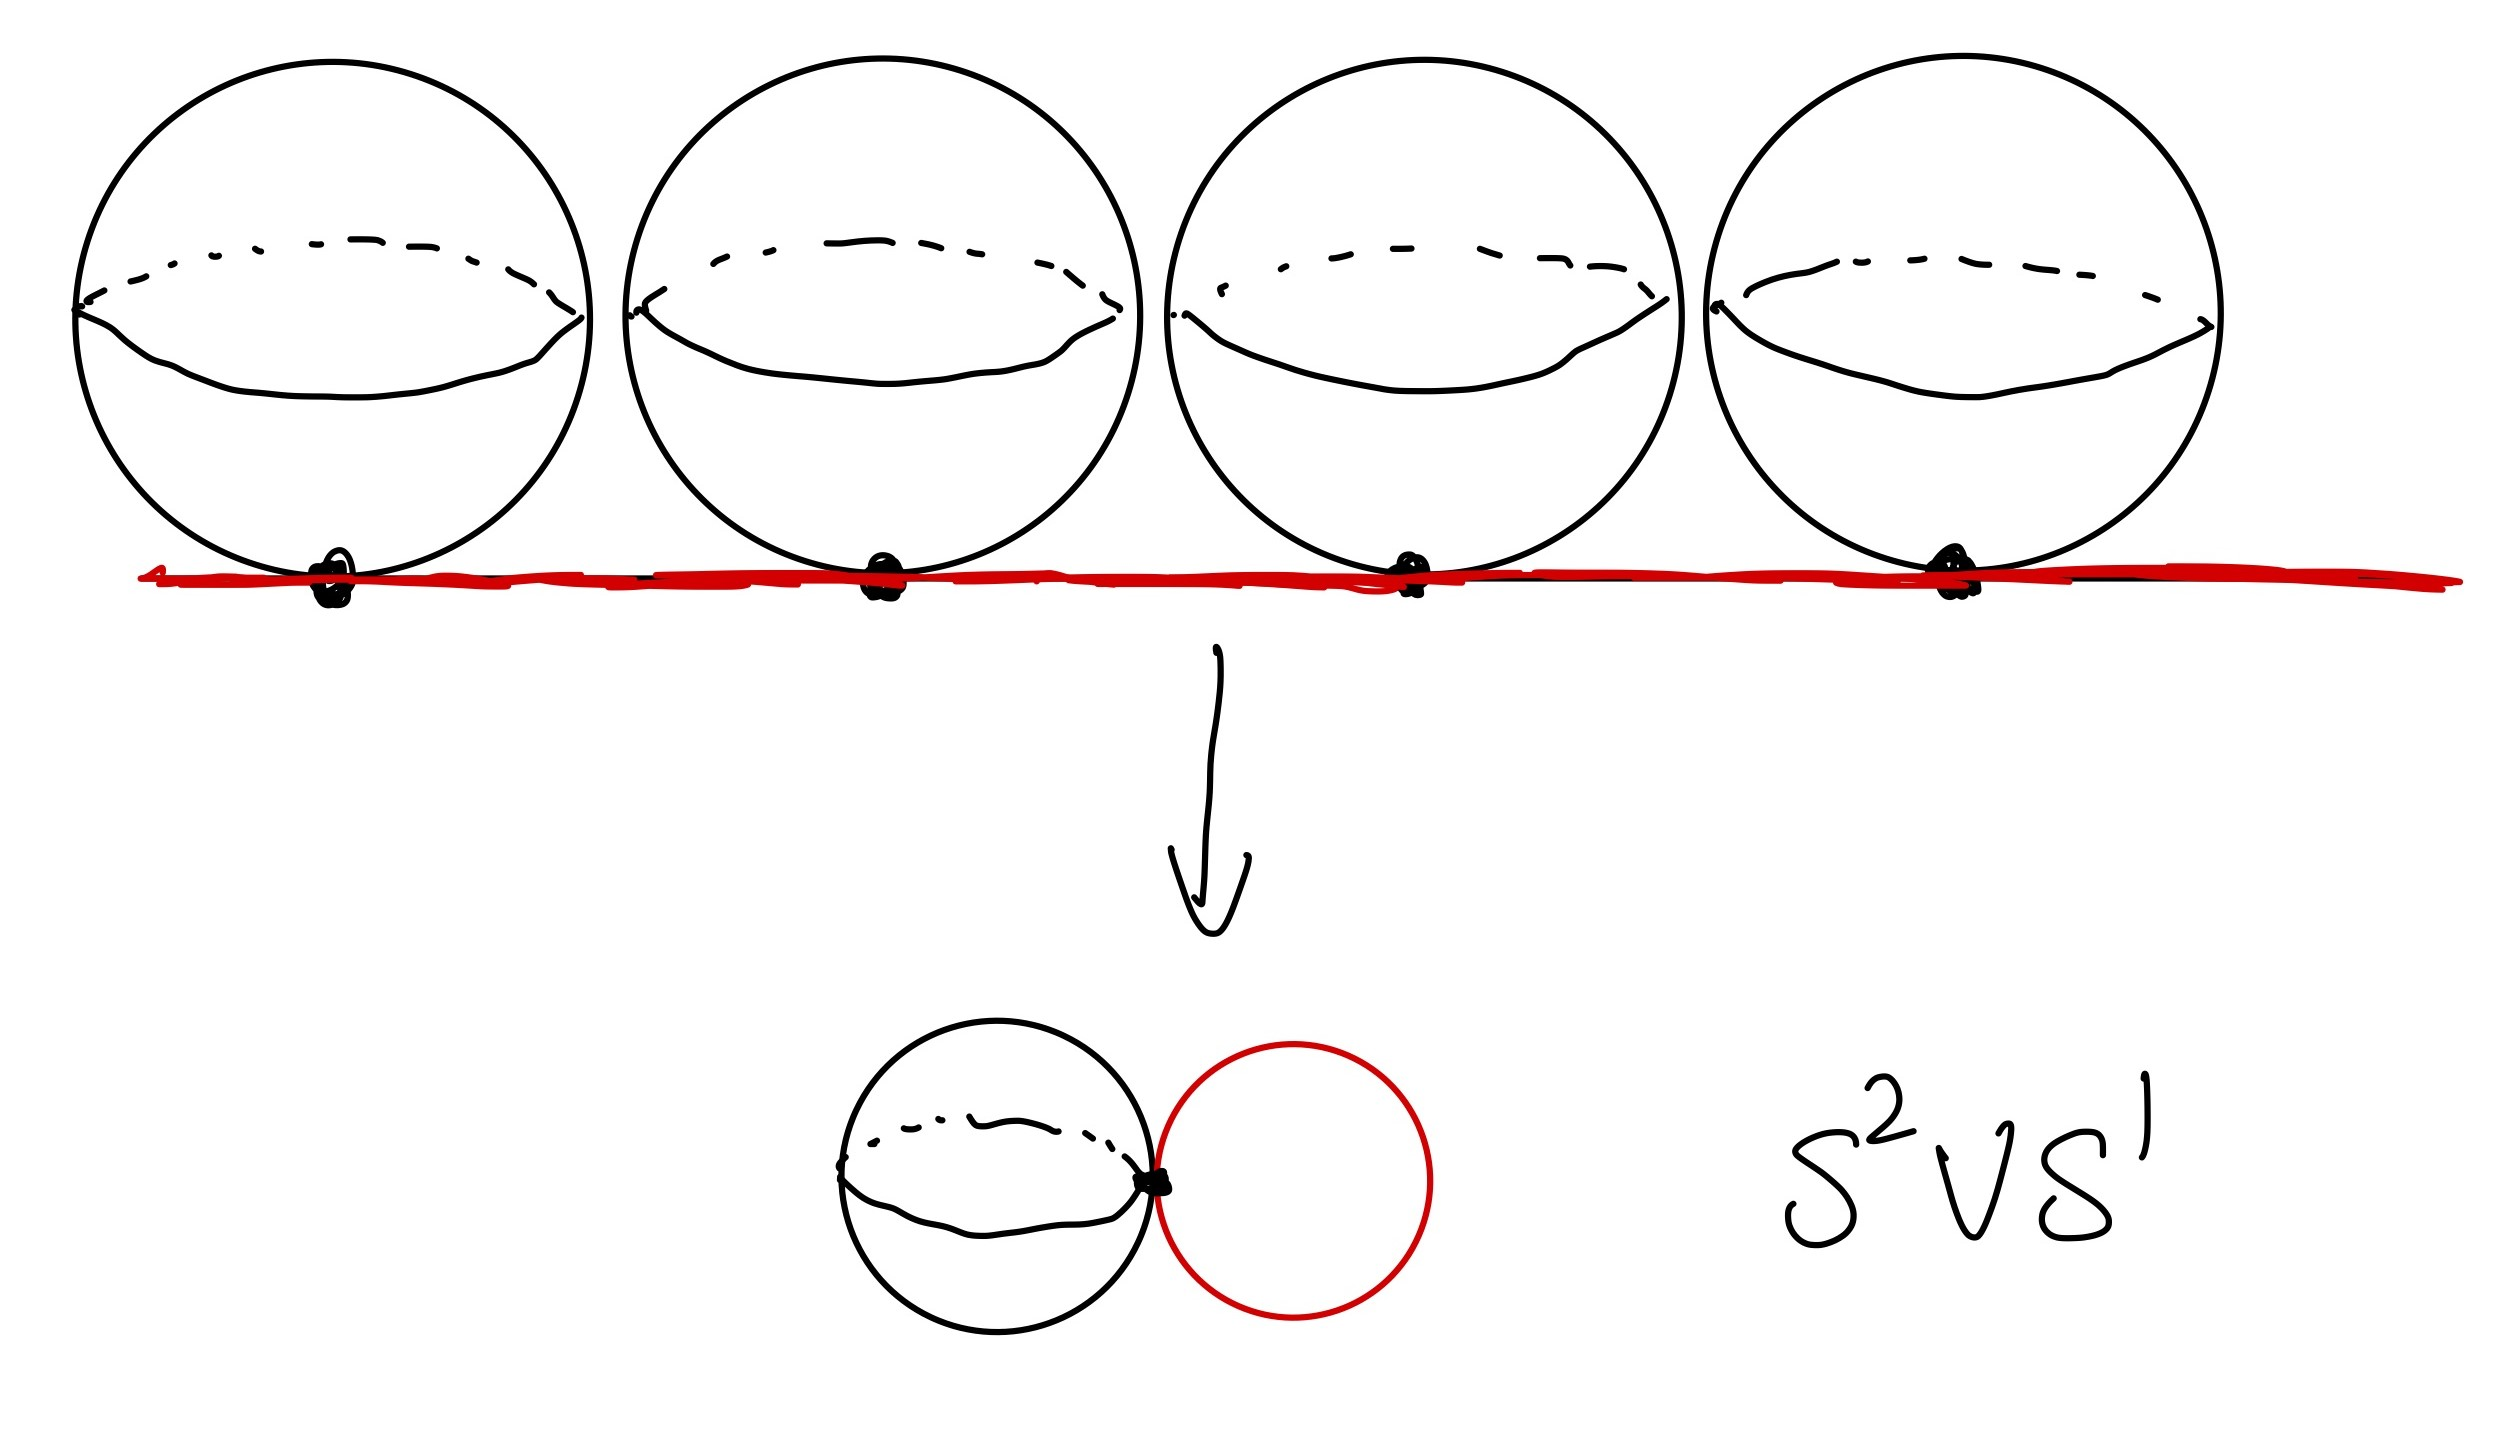
\includegraphics[scale=0.1]{Pictures/HW8-3-1.jpg}\]
This is the universal covering of \(\mathbb{R}P^2\vee \mathbb{R}P^2\), we have infinitely many spheres wedged together in the way shown below. 
\[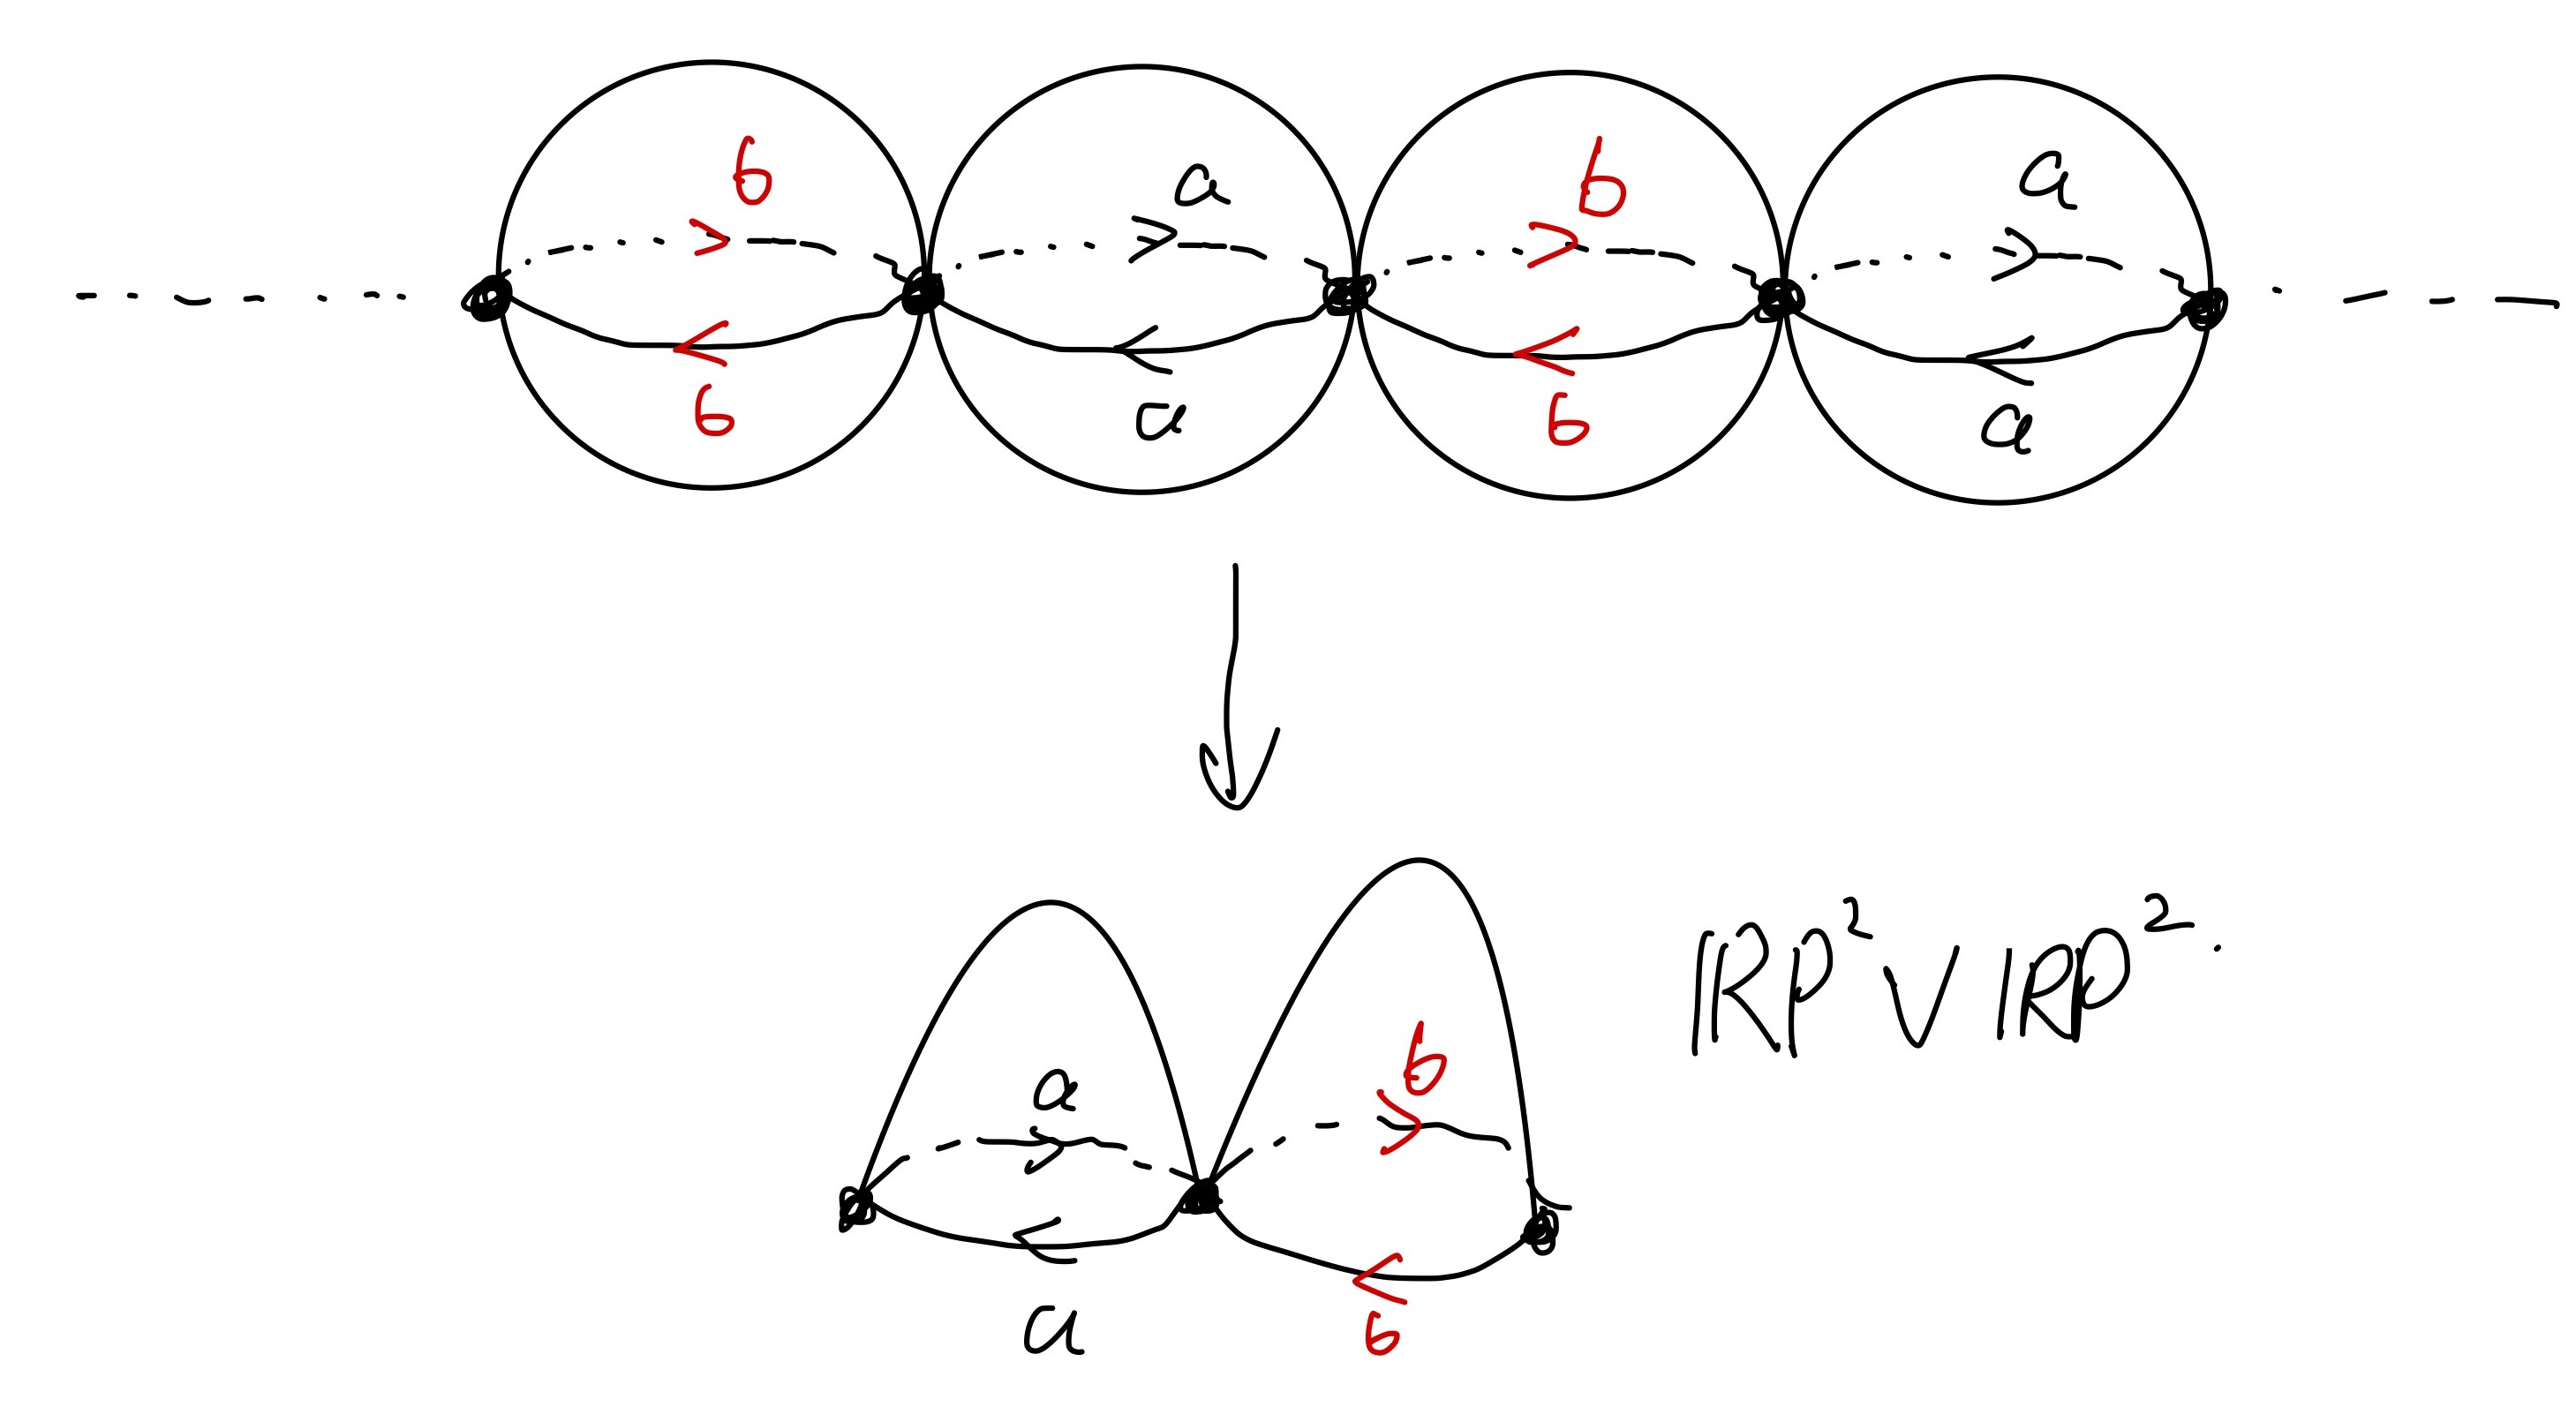
\includegraphics[scale=0.1]{Pictures/HW8-3-2.jpg}\]
This is the universal covering of \(\mathbb{R}P^2\vee S^2\). This is only three spheres wedged together. 
\[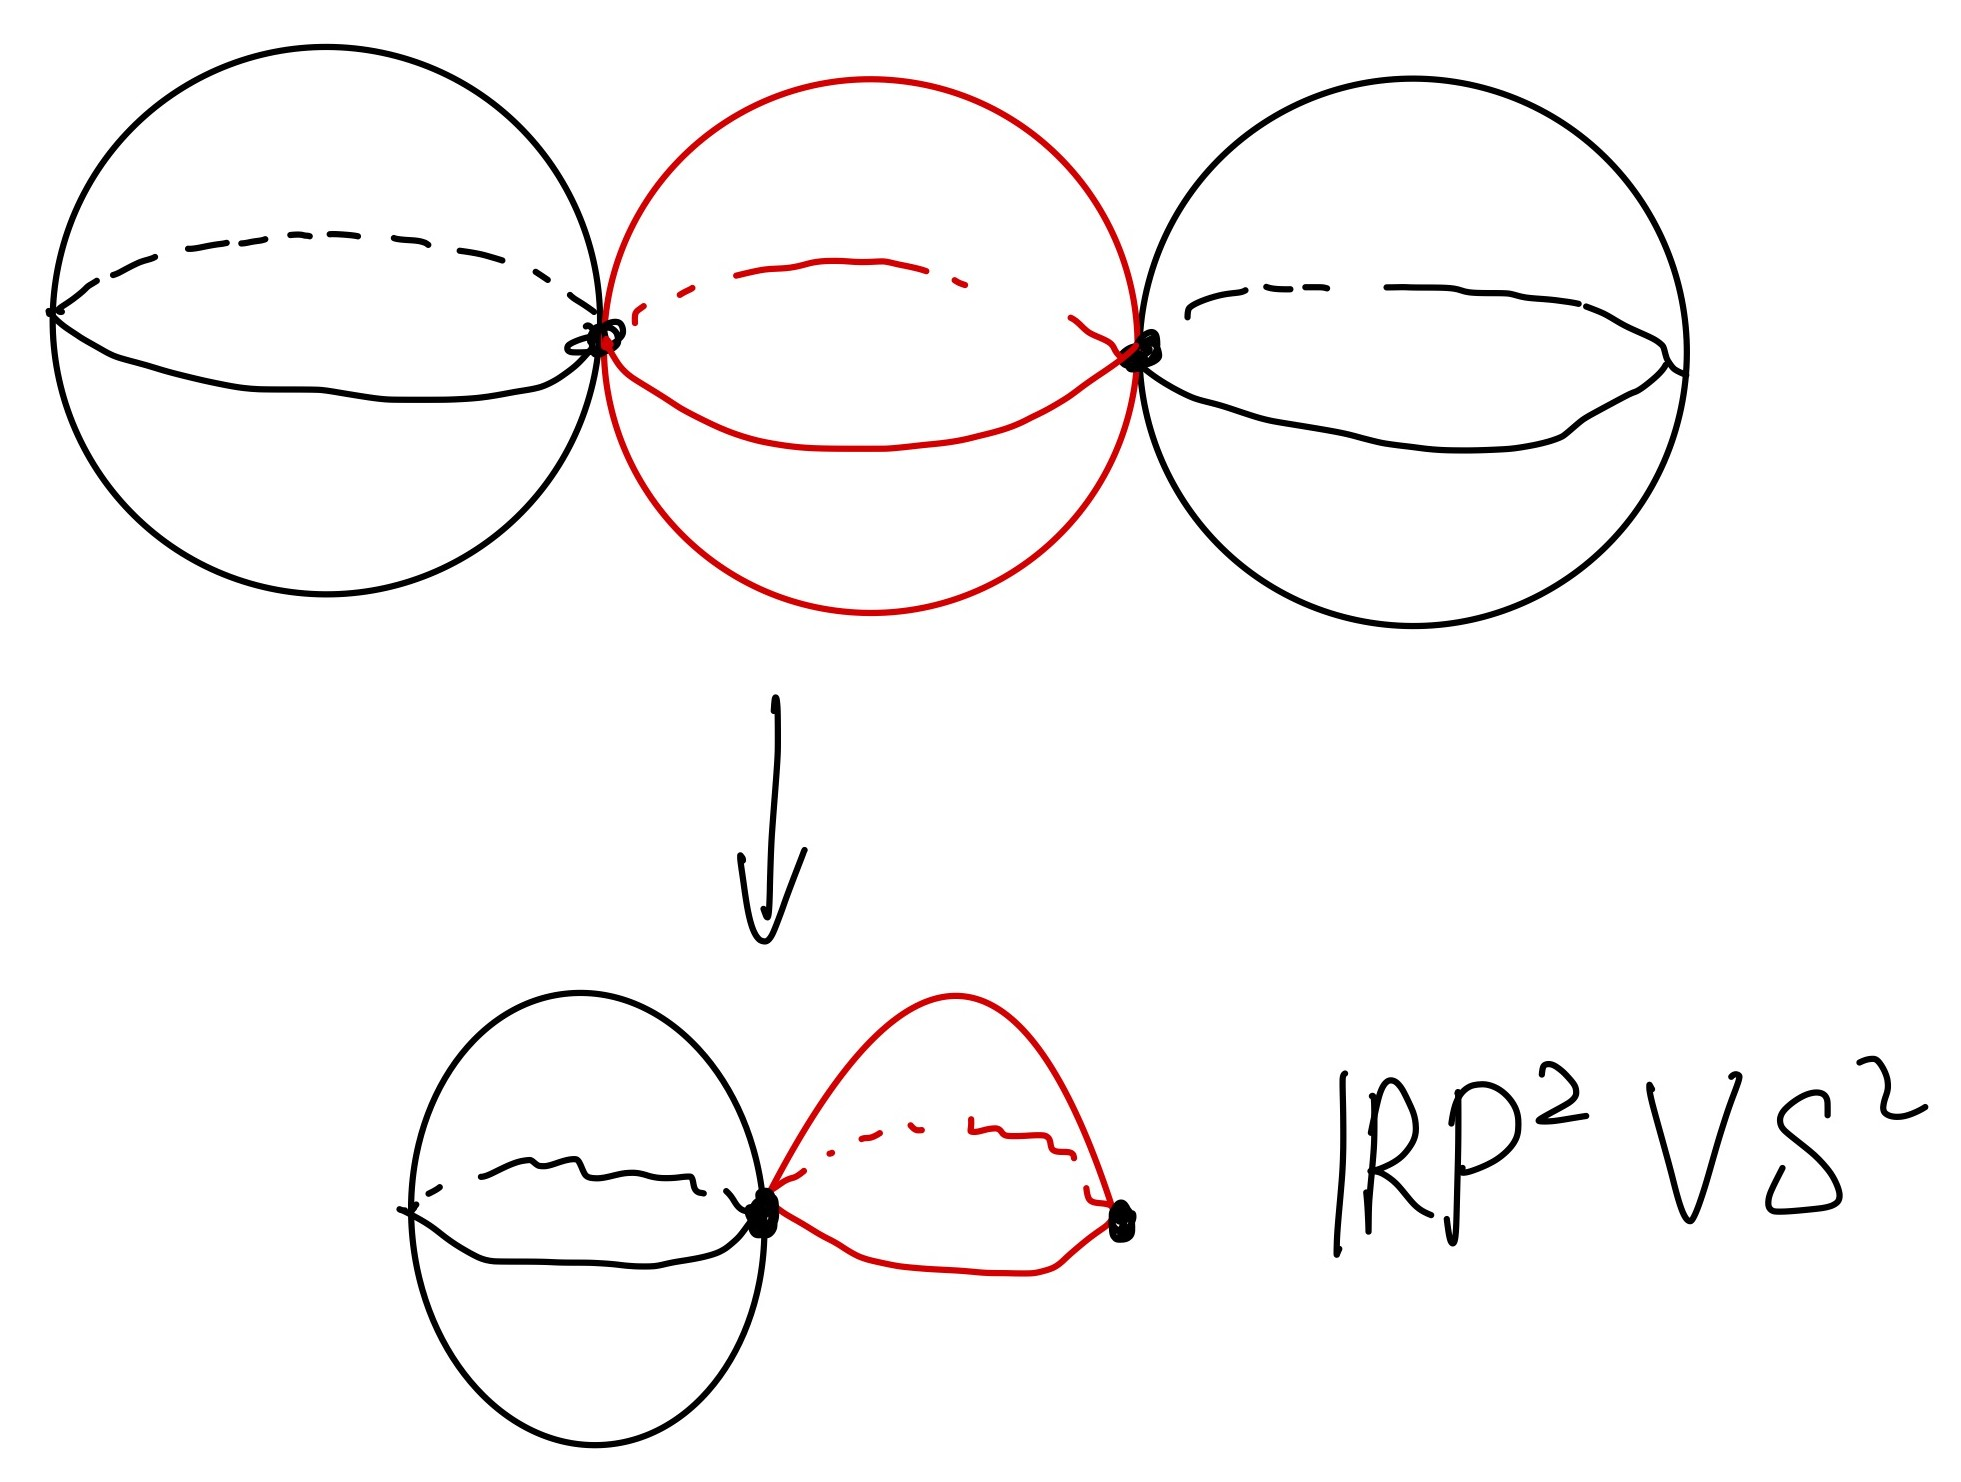
\includegraphics[scale=0.1]{Pictures/HW8-3-3.jpg}\]
This is the universal covering of \(\mathbb{R}P^2\vee S^1\). 
\[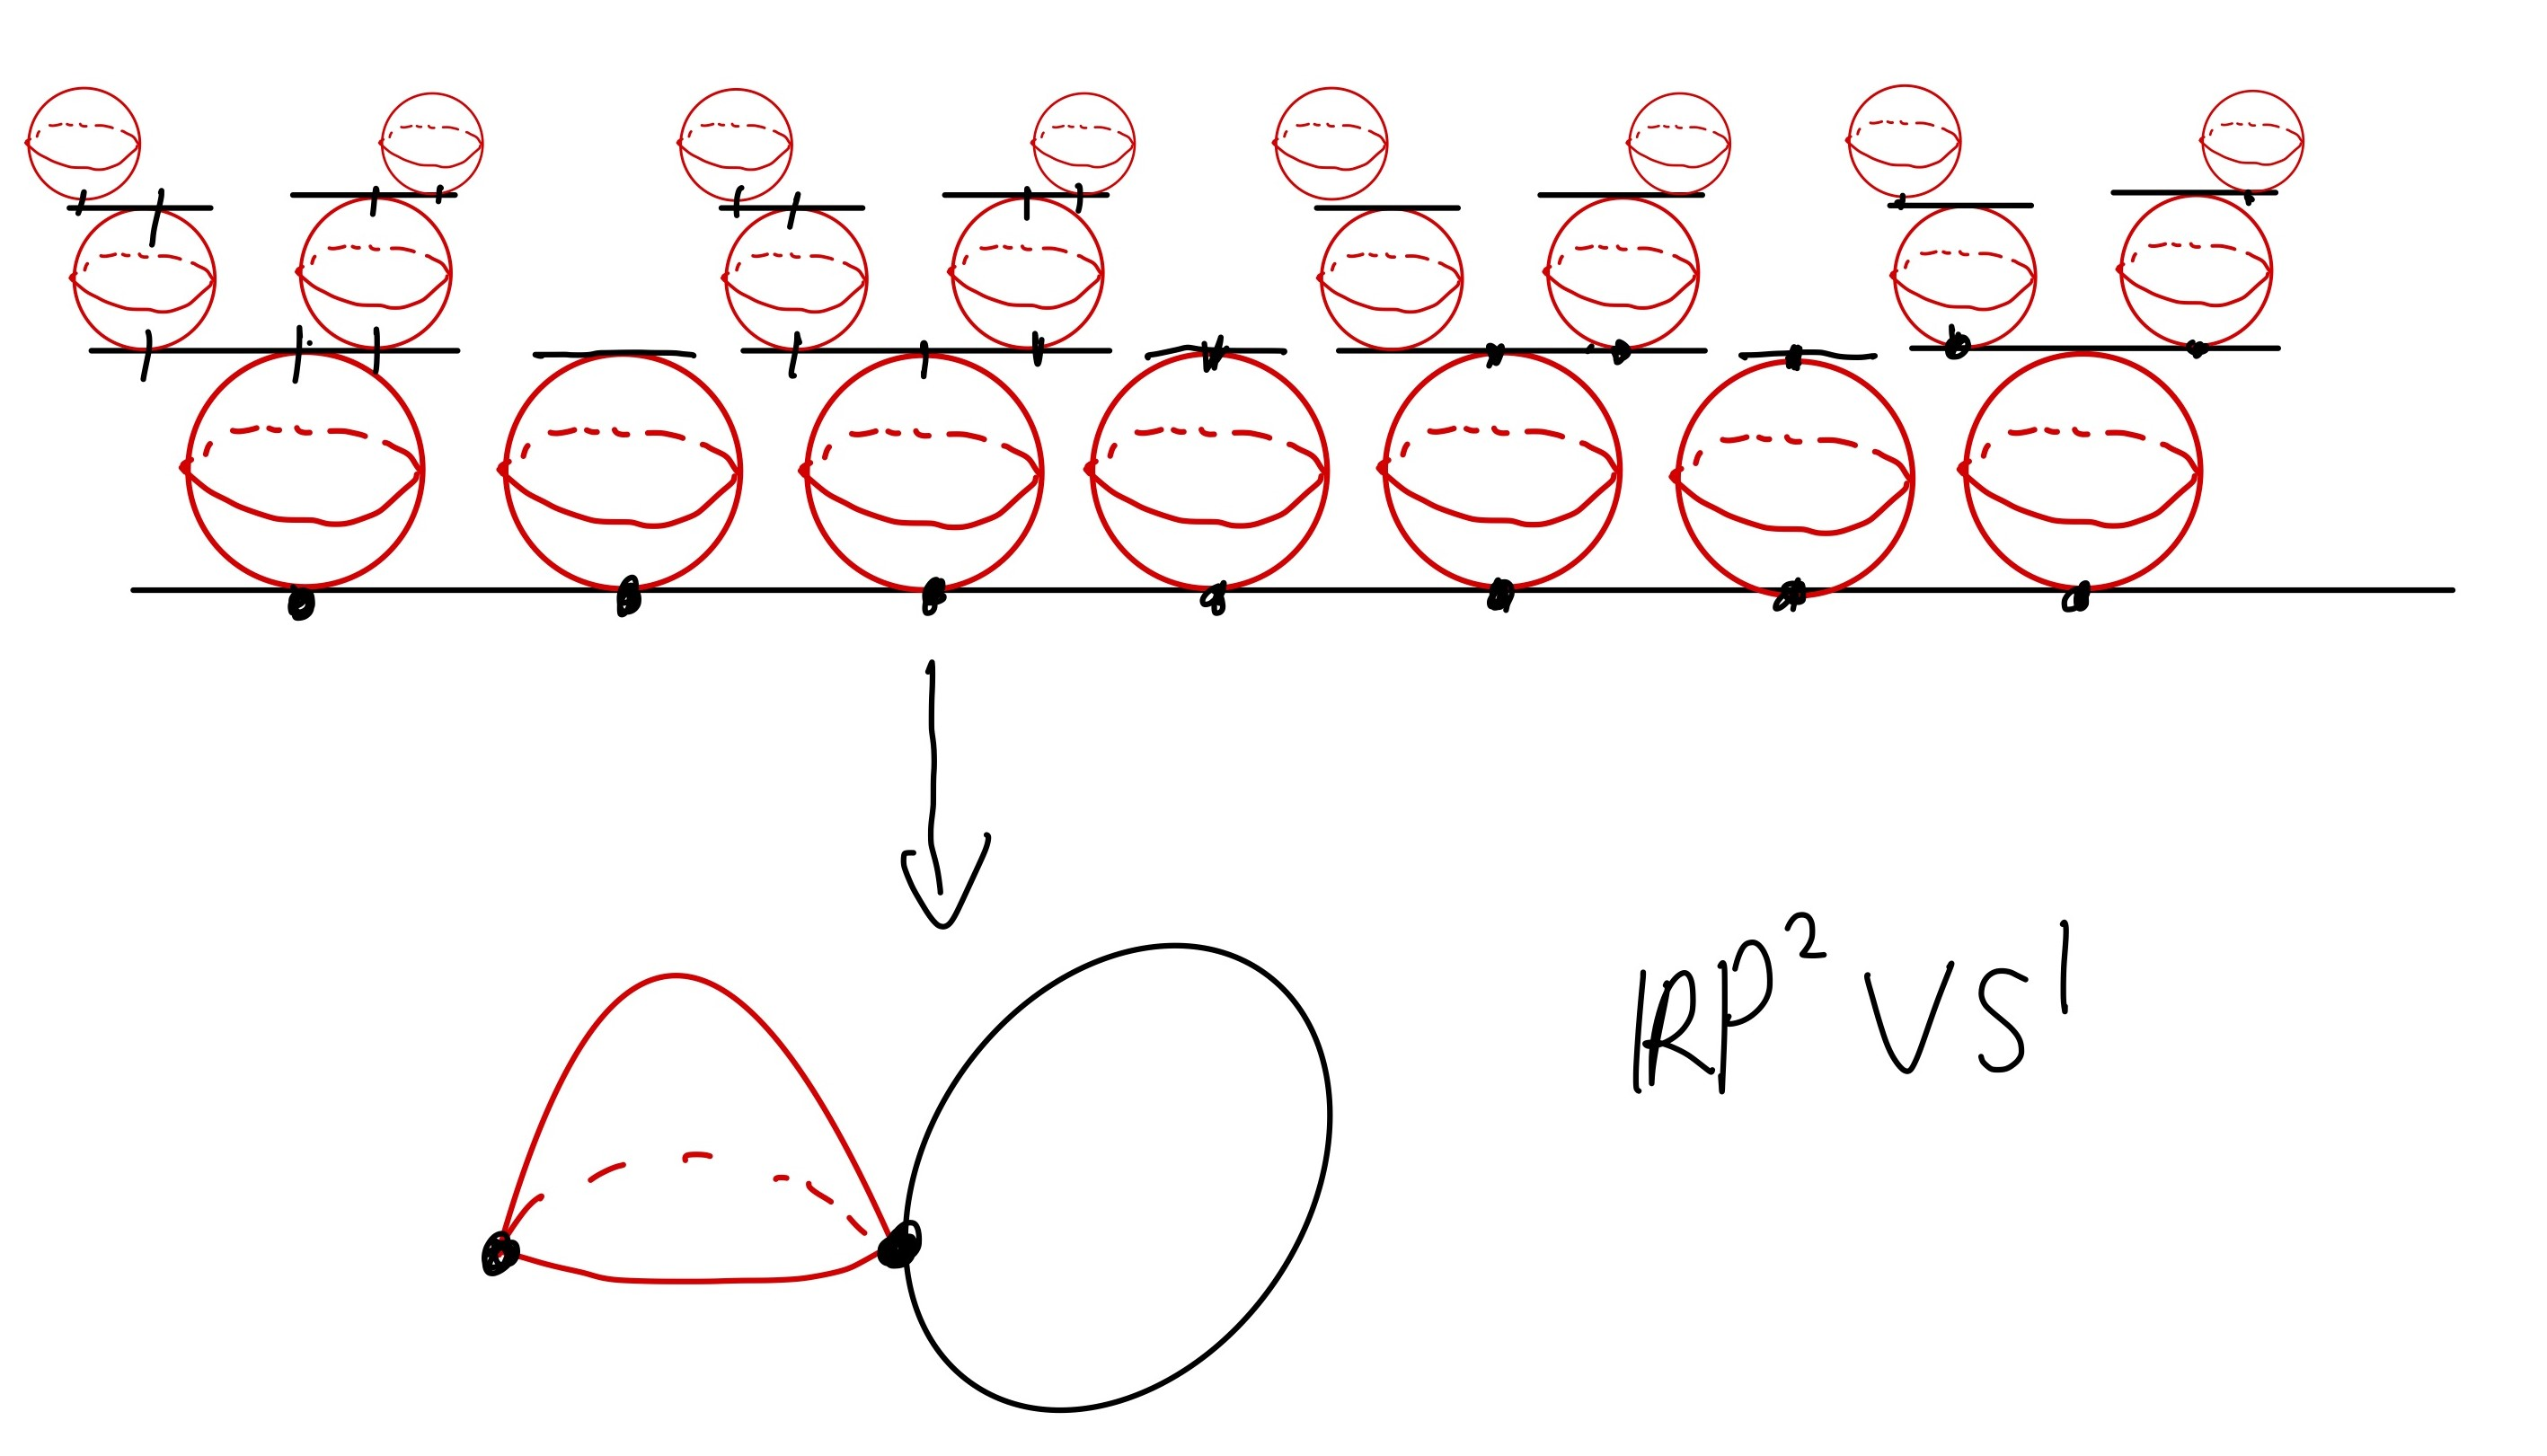
\includegraphics[scale=0.1]{Pictures/HW8-3-4.jpg}\]
\item Let 
\[G=\pi_1(\mathbb{R}P^2\vee \mathbb{R}P^2)=\mathbb{Z}/2 \mathbb{Z}*\mathbb{Z}/2 \mathbb{Z}=\la a,b\mid a^2=b^2=1\ra.\]
By the classification theorem for covering spaces, we need to find transitive left \(G\)-set. We have only one connected Cayley Graph of size \(3\):
% https://q.uiver.app/#q=WzAsMyxbMCwwLCJzXzEiXSxbMiwwLCJzXzIiXSxbMSwyLCJzXzMiXSxbMCwxLCJhIl0sWzEsMCwiYSIsMCx7Im9mZnNldCI6LTN9XSxbMSwyLCJiIiwwLHsiY29sb3VyIjpbMCw2MCw2MF19LFswLDYwLDYwLDFdXSxbMiwxLCJiIiwwLHsib2Zmc2V0IjotMywiY29sb3VyIjpbMCw2MCw2MF19LFswLDYwLDYwLDFdXSxbMCwwLCJiIiwwLHsiYW5nbGUiOi05MCwiY29sb3VyIjpbMCw2MCw2MF19LFswLDYwLDYwLDFdXSxbMiwyLCJhIiwwLHsiYW5nbGUiOi0xMzV9XV0=
\[\begin{tikzcd}
	{s_1} && {s_2} \\
	\\
	& {s_3}
	\arrow["b", color={rgb,255:red,214;green,92;blue,92}, from=1-1, to=1-1, loop, in=145, out=215, distance=10mm]
	\arrow["a", from=1-1, to=1-3]
	\arrow["a", shift left=3, from=1-3, to=1-1]
	\arrow["b", color={rgb,255:red,214;green,92;blue,92}, from=1-3, to=3-2]
	\arrow["b", shift left=3, color={rgb,255:red,214;green,92;blue,92}, from=3-2, to=1-3]
	\arrow["a", from=3-2, to=3-2, loop, in=190, out=260, distance=10mm]
\end{tikzcd}\]
We can see the stabilizer
\[\Stab(s_1)=\la b, ababa\ra.\]
Let \(\ti{B}\) be the universal covering shown in the picture above. We first try find out what is \(\ti{B}/\la b\ra\). 
\[\includegraphics[scale=0.1]{Pictures/Hw8-3-5.jpg}\]
We can see that by quotient out the subgroup generated by \(b\), the space becomes half of what we begin with (the half sphere is homeomorphic to \(\mathbb{R}P^2\)). Using a similar argument 
we can see that 
\[\includegraphics[scale=0.1]{Pictures/Hw8-3-6.jpg}\]
So the 3-fold path-connected covering of \(\mathbb{R}P^2\vee \mathbb{R}P^2\) is homeomorphic to \(\mathbb{R}P^2\vee S^2\vee S^2\vee \mathbb{R}P^2\). This is the only one.
\end{enumerate}
\end{solution}

\noindent\rule{7in}{2.8pt}
%%%%%%%%%%%%%%%%%%%%%%%%%%%%%%%%%%%%%%%%%%%%%%%%%%%%%%%%%%%%%%%%%%%%%%%%%%%%%%%%%%%%%%%%%%%%%%%%%%%%%%%%%%%%%%%%%%%%%%%%%%%%%%%%%%%%%%%%
%Probelm 4
%%%%%%%%%%%%%%%%%%%%%%%%%%%%%%%%%%%%%%%%%%%%%%%%%%%%%%%%%%%%%%%%%%%%%%%%%%%%%%%%%%%%%%%%%%%%%%%%%%%%%%%%%%%%%%%%%%%%%%%%%%%%%%%%%%%%%%%%
\begin{problem}{4}
\begin{enumerate}[(a)]
\item Let \(p:E\rightarrow B\) be a \(k\)-fold covering space, and let \(U\hookrightarrow B\) be an open cell (a subset homeomorphic to \(\mathbb{R}^n\), for some \(n\)). Prove that \(p^{-1}(U)\) consists of \(k\) disjoint copies of \(U\). 
\item  If \(B\) has a CW filtration, \(B_0\subseteq B_1\subseteq \cdots \subseteq B\), there is a resulting filtration 
\[p^{-1}(B_0)\subseteq p^{-1}(B_1)\subseteq \cdots \subseteq E\]
Explain why \(p^{-1}(B_i)\setminus p^{-1}(B_{i-1})\) is a disjoint union of open \(i\)-cells, for each \(i\). 
\item Recall that a finite CW complex has an Euler characteristic, equal to the alternating sum of the number of cells. If \(B\) is a finite CW complex, so is \(E\). How does 
\(\chi(E)\) relate to \(\chi(B)\)? 
\item Fix \(n\geq 1\). Answer the following three questions, with explanations: 
\begin{enumerate}[i.]
\item Can be Klein bottle b finitely (and evenly) covered by a genus \(2\) orientable surface? 
\item Does \(S^{2n}\) have a path-connected \(3\)-fold covering space? 
\item Is \(S^{2n}\) a \(3\)-fold covering of some other space \(X\)?
\end{enumerate} 
\end{enumerate}
\end{problem}
\begin{solution}
\begin{enumerate}[(a)]
\item We first prove a fact. 
\begin{claim}
The map \(p:p^{-1}(U)\rightarrow U\) is also a covering space.
\end{claim}
\begin{claimproof}
Let \(x\in U\) and the discrete set \(F\) be the fiber. There exists an open set \(V\subseteq B\) such that \(V\times F\) is homeomorphic to \(p^{-1}(V)\). Consider the open set \(V\cap U\) in \(U\). We know that 
\(p^{-1}(U\cap V)\subset p^{-1}(V)\cong V\times F\). We have a commutative diagram 
% https://q.uiver.app/#q=WzAsMyxbMCwwLCJwXnstMX0oVikiXSxbMSwwLCJWXFx0aW1lcyBGIl0sWzAsMSwiViJdLFswLDIsInAiLDJdLFswLDEsIlxcY29uZyJdLFsxLDIsIlxccGlfMSJdXQ==
\[\begin{tikzcd}
	{p^{-1}(V)} & {V\times F} \\
	V
	\arrow["\cong", from=1-1, to=1-2]
	\arrow["p"', from=1-1, to=2-1]
	\arrow["{\pi_1}", from=1-2, to=2-1]
\end{tikzcd}\]
Since \(F\) is discrete, then \(p^{-1}(V\cap U)\cong (U\cap V)\times F\), which is compatible with projection to \(V\cap U\). This proves \(p^{-1}(U)\rightarrow U\) is a covering space. 
\end{claimproof}

Note that \(U\cong \mathbb{R}^n\) is simply connected, so the homeomorphism \(U\rightarrow U\) is the universal covering. By the classification theorem of covering space, we know that \(p^{-1}(U)\) can be written as \(\sqcup U/H_i\) where \(H_i\) is a subgroup 
of \(\pi_1(U)\), since \(\pi_1(U)\) is trivial, we know that \(p^{-1}(U)\rightarrow U\) can be written as \(\sqcup U\rightarrow U\). This is a \(k\)-fold covering, so we know that the preimage of \(U\) is disjoint \(k\) copies of \(U\).
\item For all \(i\), note that \(B_i\setminus B_{i-1}\) is the interior of all closed \(i\)-cells, which are open \(i\)-cells. From (a), we know that 
\[p^{-1}(B_i)\setminus p^{-1}(B_{i-1})=p^{-1}(B_i\setminus B_{i-1})\]
are just disjoint copies of open \(i\)-cells. 
\item We know that 
\[p^{-1}(B_0)\subseteq p^{-1}(B_1)\subseteq \cdots \subseteq E\]
is the CW filtration of \(E\). So for every \(i\)-cell in \(B\), \(E\) has \(k\) \(i\)-cells. Thus, we have 
\[\chi(E)=k\chi(B).\]
\item \begin{enumerate}[i.]
\item Let \(K\) denote the Klein bottle and \(X\) be a orientable genus 2 surface. We know that 
\(\chi(K)=0\) but \(\chi(X)=2-2g=-2\). 
Form (c) we know that \(X\) cannot be a cover of \(K\). 
\item We know that \(S^{2n}\) is simply connected, so for any 3-fold covering map \(p:E\rightarrow S^{2n}\), \(E\) must be disjoint union of 3 copies of \(S^{2n}\). So this cannot be path-connected. 
\item We know that \(\chi(S^{2n})=1+1=2\), which is not divisible by \(3\). So \(S^{2n}\) cannot be a 3-fold covering of other space.
\end{enumerate}

\end{enumerate}
\end{solution}

\noindent\rule{7in}{2.8pt}
%%%%%%%%%%%%%%%%%%%%%%%%%%%%%%%%%%%%%%%%%%%%%%%%%%%%%%%%%%%%%%%%%%%%%%%%%%%%%%%%%%%%%%%%%%%%%%%%%%%%%%%%%%%%%%%%%%%%%%%%%%%%%%%%%%%%%%%%
%Probelm 5 Klein bottle
%%%%%%%%%%%%%%%%%%%%%%%%%%%%%%%%%%%%%%%%%%%%%%%%%%%%%%%%%%%%%%%%%%%%%%%%%%%%%%%%%%%%%%%%%%%%%%%%%%%%%%%%%%%%%%%%%%%%%%%%%%%%%%%%%%%%%%%
\begin{problem}{5}
Let \(K\) denote the Klein bottle. Recall that \(\pi_1(K)=\la a,b\mid aba=b\ra\).
\begin{enumerate}[(1)]
\item How many path-connected \(2\)-fold coverings does \(K\) have (up to isomorphism)? Try to draw pictures depicting them. For each of these \(2\)-fold covering \(E\rightarrow K\), determine what familiar \(2\)-manifold \(E\) is homeomorphic to. 
\item Repeat part (a) for the \(3\)-fold covering spaces of \(K\). 
\end{enumerate}
\end{problem}
\begin{solution}
\begin{enumerate}[(2)]
\item Let \(G=\pi_1(K)\). By the classification theorem for coverings, to find all the path-connected \(2\)-fold coverings, we need to find all transitive \(G\)-sets of sizes. It is the same as find all the connected Cayley Graph of size \(2\). We have the following three graphs:
\begin{figure}[h]
\begin{subfigure}{0.32\textwidth}
\centering
% https://q.uiver.app/#q=WzAsMixbMCwwLCJzXzEiXSxbMSwwLCJzXzIiXSxbMCwxLCJhIiwwLHsiY3VydmUiOi0yfV0sWzEsMCwiYSIsMCx7ImN1cnZlIjotMn1dLFswLDAsImIiLDAseyJhbmdsZSI6LTkwLCJjb2xvdXIiOlswLDYwLDYwXX0sWzAsNjAsNjAsMV1dLFsxLDEsImIiLDAseyJhbmdsZSI6OTAsImNvbG91ciI6WzAsNjAsNjBdfSxbMCw2MCw2MCwxXV1d
\begin{tikzcd}
	{s_1} & {s_2}
	\arrow["b", color={rgb,255:red,214;green,92;blue,92}, from=1-1, to=1-1, loop, in=145, out=215, distance=10mm]
	\arrow["a", curve={height=-12pt}, from=1-1, to=1-2]
	\arrow["a", curve={height=-12pt}, from=1-2, to=1-1]
	\arrow["b", color={rgb,255:red,214;green,92;blue,92}, from=1-2, to=1-2, loop, in=325, out=35, distance=10mm]
\end{tikzcd}
\caption{}
\end{subfigure}
\begin{subfigure}{0.32\textwidth}
\centering
% https://q.uiver.app/#q=WzAsMixbMCwwLCJzXzEiXSxbMSwwLCJzXzIiXSxbMCwxLCJiIiwwLHsiY3VydmUiOi0yLCJjb2xvdXIiOlswLDYwLDYwXX0sWzAsNjAsNjAsMV1dLFsxLDAsImIiLDAseyJjdXJ2ZSI6LTIsImNvbG91ciI6WzAsNjAsNjBdfSxbMCw2MCw2MCwxXV0sWzAsMCwiYSIsMCx7ImFuZ2xlIjotOTB9XSxbMSwxLCJhIiwwLHsiYW5nbGUiOjkwfV1d
\begin{tikzcd}
	{s_1} & {s_2}
	\arrow["a", from=1-1, to=1-1, loop, in=145, out=215, distance=10mm]
	\arrow["b", color={rgb,255:red,214;green,92;blue,92}, curve={height=-12pt}, from=1-1, to=1-2]
	\arrow["b", color={rgb,255:red,214;green,92;blue,92}, curve={height=-12pt}, from=1-2, to=1-1]
	\arrow["a", from=1-2, to=1-2, loop, in=325, out=35, distance=10mm]
\end{tikzcd}
\caption{}
\end{subfigure}
\begin{subfigure}{0.32\textwidth}
\centering
% https://q.uiver.app/#q=WzAsMixbMCwwLCJzXzEiXSxbMSwwLCJzXzIiXSxbMCwxLCJiIiwwLHsiY3VydmUiOi0yLCJjb2xvdXIiOlswLDYwLDYwXX0sWzAsNjAsNjAsMV1dLFsxLDAsImIiLDAseyJjdXJ2ZSI6LTIsImNvbG91ciI6WzAsNjAsNjBdfSxbMCw2MCw2MCwxXV0sWzAsMSwiYSIsMCx7ImN1cnZlIjotNX1dLFsxLDAsImEiLDAseyJjdXJ2ZSI6LTV9XV0=
\begin{tikzcd}
	{s_1} & {s_2}
	\arrow["b", color={rgb,255:red,214;green,92;blue,92}, curve={height=-12pt}, from=1-1, to=1-2]
	\arrow["a", curve={height=-30pt}, from=1-1, to=1-2]
	\arrow["b", color={rgb,255:red,214;green,92;blue,92}, curve={height=-12pt}, from=1-2, to=1-1]
	\arrow["a", curve={height=-30pt}, from=1-2, to=1-1]
\end{tikzcd}
\caption{}
\end{subfigure}
\end{figure}
We calculate the stabilizers in each of these Cayley Graphs:
\begin{align*}
	(a)&\ \ \Stab(s_1)=\Stab(s_2)=\la a^2,b\ra,\\
	(b)&\ \ \Stab(s_1)=\Stab(s_2)=\la a,b^2\ra,\\
	(c)&\ \ \Stab(s_1)=\Stab(s_2)=\la a^2,b^2,ab\ra.\\
\end{align*}
The Klein bottle has the following CW complex structure 
\[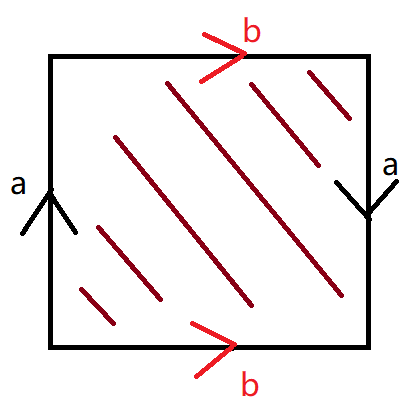
\includegraphics[scale=0.5]{Pictures/HW8-5-1.png}\]
where the fundamental group is generated by the homotopy classes of two \(1\)-cells \(a\) and \(b\). The universal covering space is given by the map \(p:\mathbb{R}^2\rightarrow K\) as shown in the picture: 
\[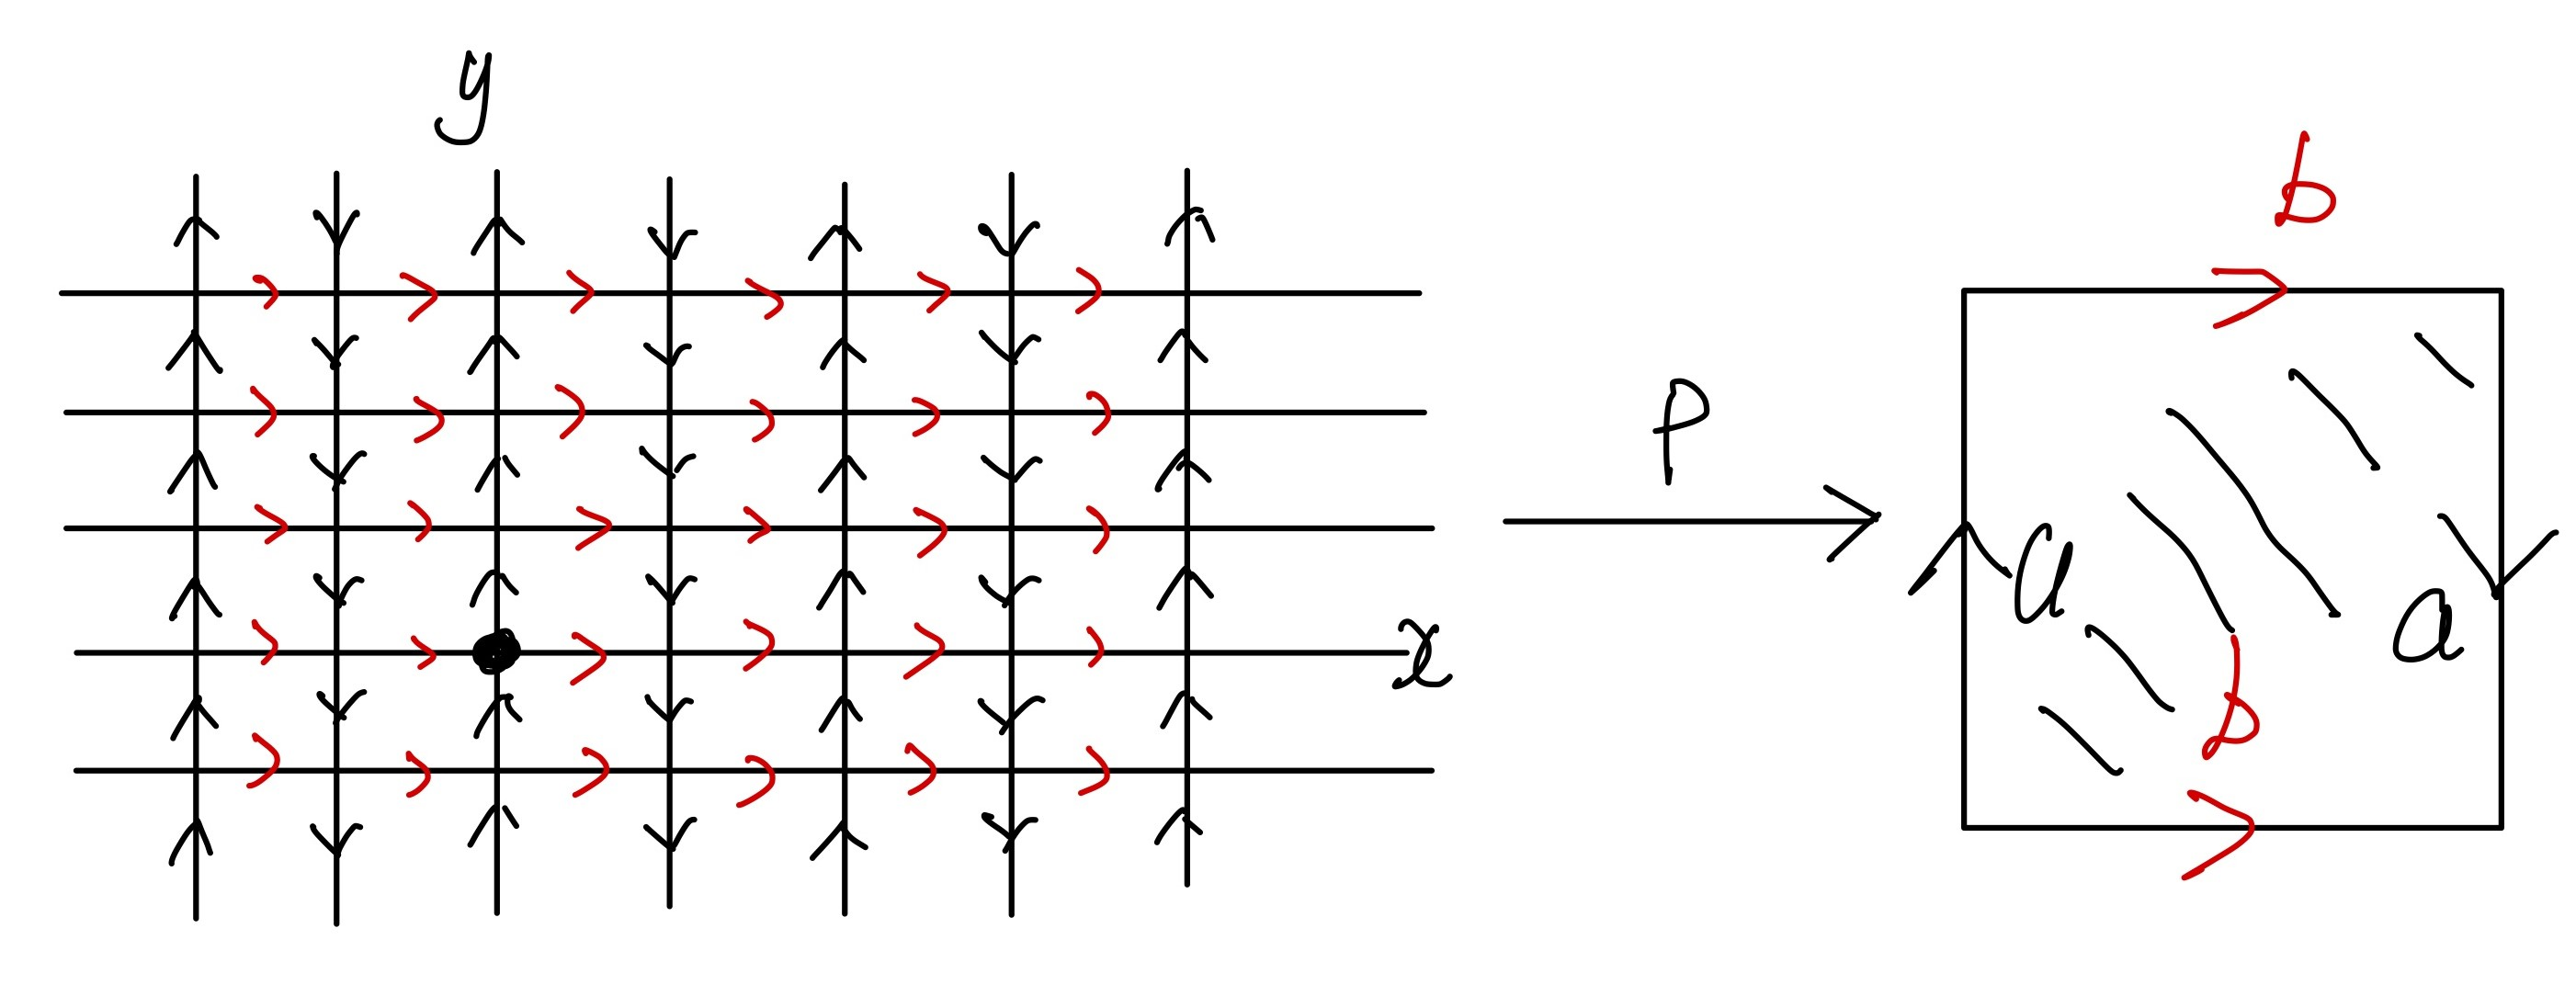
\includegraphics[scale=0.1]{Pictures/HW8-5-2.jpg}\]
For convenience, we choose the base point in \(\mathbb{R}^2\) as \((0,0)\) and establish a coordinate system. Let \(b\in K\) be the \(0\)-cell, viewed as the base point in \(K\). \(p^{-1}(b)\) is the set of all integer points 
in \(\mathbb{R}^2\). To understand how the group acts on \(\mathbb{R}^2\), we need to understand how the point \((x,y)\) in the grid formed by the integer points moves along the path \(a\) and \(b\). 
When \(x\) is an even integer, following the path \(a\) is adding a positive number to the \(y\) coordiante, and when \(x\) is an odd integer, following the path \(a\) is substracting a positive number in the \(y\) coordinates. We discuss covering spaces corresponding to the picture \((a)\), \((b)\) and \((c)\).
\begin{enumerate}[(a)]
\item We consider the orbit space of \(\mathbb{R}^2\) under the action of subgroup generated by \(a^2,b\). We first quotient out \(b\). Let \((x,y)\in \mathbb{R}^2\), we need to identify points \((x,y)\sim (x,y)\cdot b\). Note that by following the path \(b\), 
we add \(1\) to the \(x\) coordiante, so we need to identify \((x,y)\sim (x+1,-y)\) for all \(x,y\in \mathbb{R}\) because we change the parity (even or odd) of \(x\). The quotient space \(\mathbb{R}^2/\la b\ra\) can be viewed as the subspace 
\[\left\{ (x,y)\in \mathbb{R}^2\mid 0\leq x\leq 1 ,(0,y)\sim (1,-y)\right\}\subseteq \mathbb{R}^2\]
where we identify \((0,y)\sim (1,-y)\) for all \(y\in \mathbb{R}\). Next, we identify points \((x,y)\sim (x,y)\cdot a^2\). Note that by following the path \(a^2\), we add \(2\) to the \(y\) coordinates. So we have 
\[\mathbb{R}^2/\la a^2,b\ra=\left\{ (x,y)\in \mathbb{R}^2\mid 0\leq x\leq 1,0\leq y\leq 2, (0,y)\sim (1,2-y), (x,0)\sim (x,2) \right\}\]
The covering space is shown as 
\[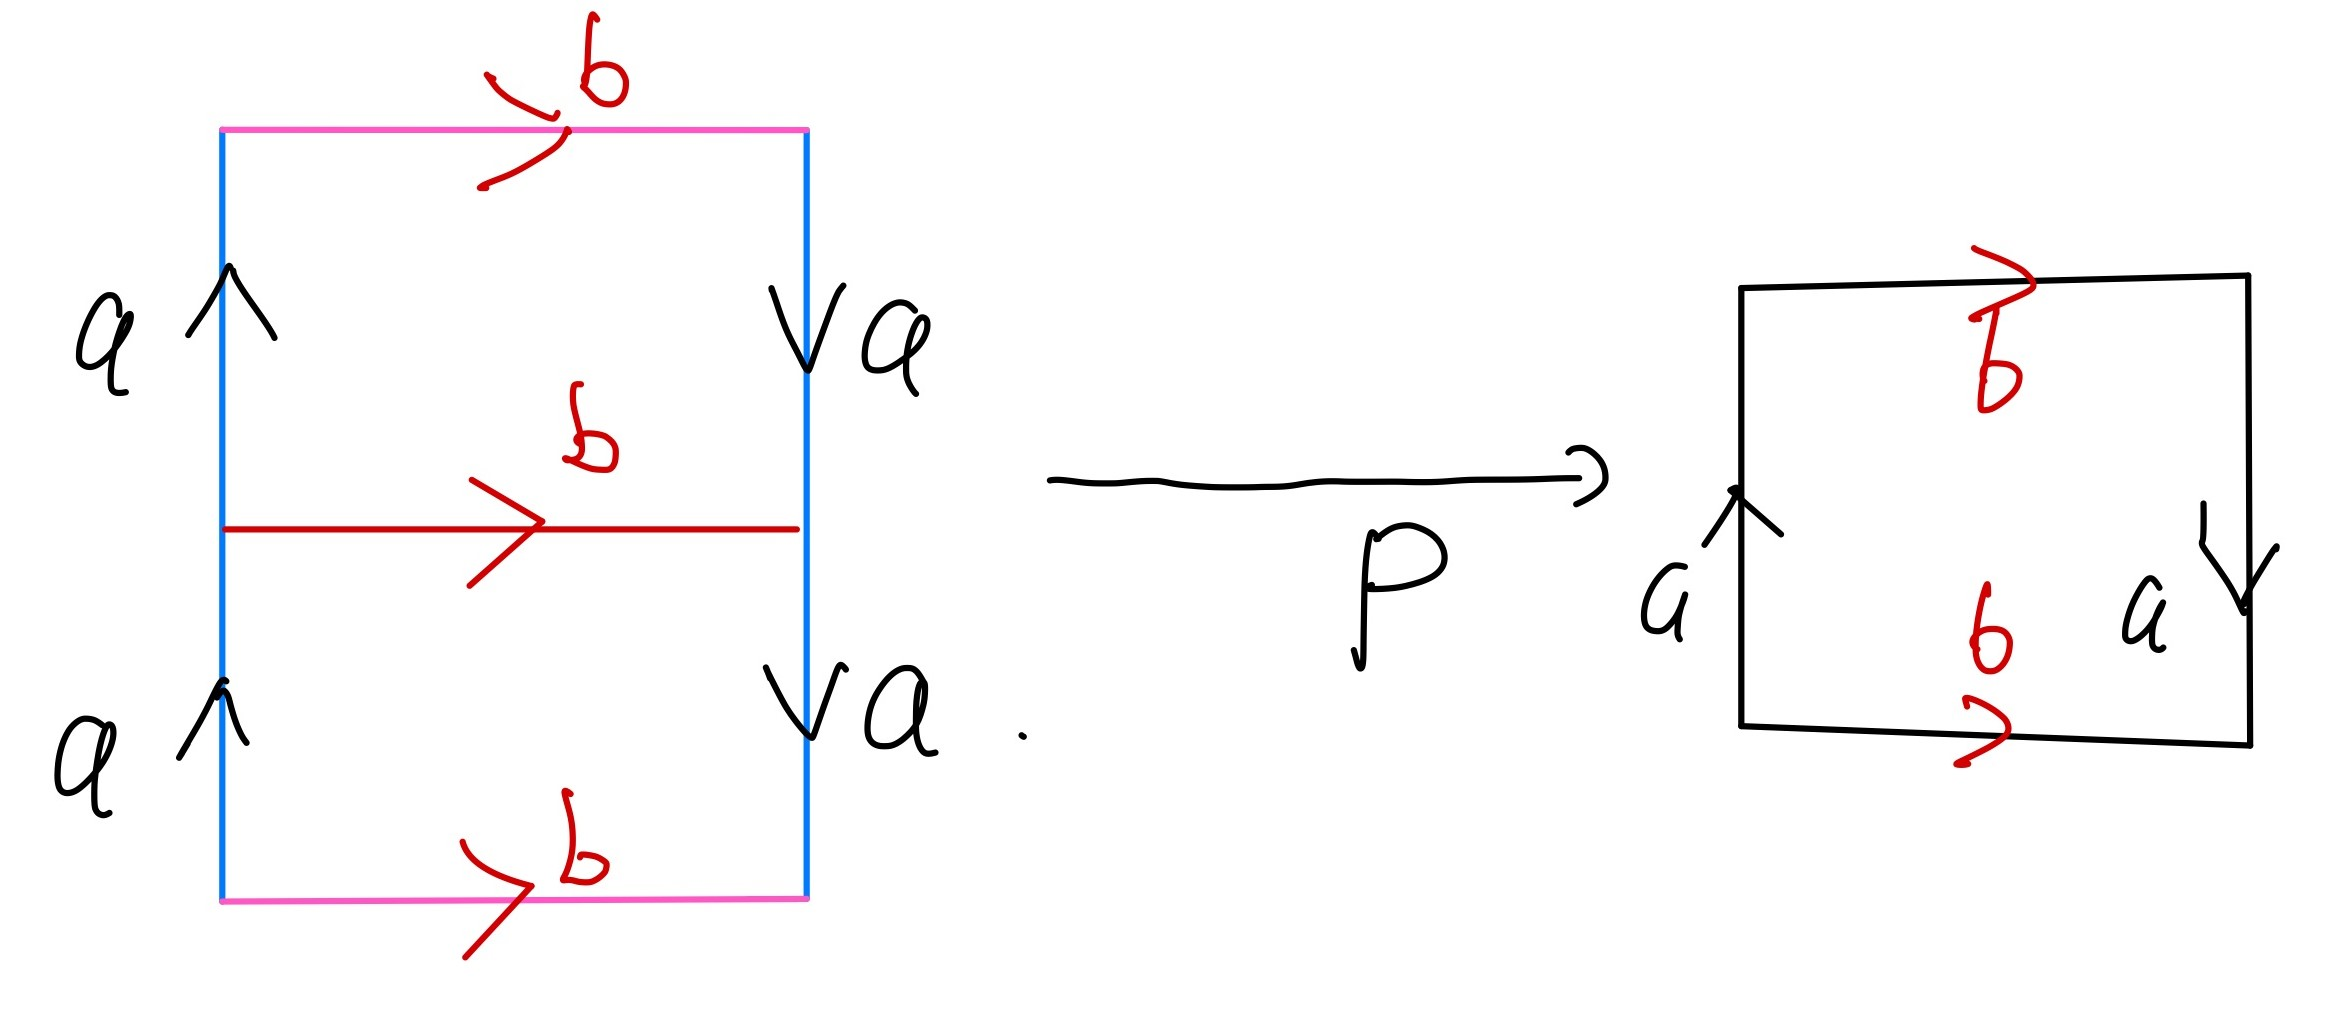
\includegraphics[scale=0.1]{Pictures/HW8-5-3.jpg}\]
The identification tells us the space is homeomorphic to the Klein bottle.
\item We consider the orbit space of \(\mathbb{R}^2\) under the action of subgroup generated by \(a,b^2\). Let \((x,y)\in \mathbb{R}^2\). Note that following by the path \(a\) is adding \(1\) to the \(y\) coordinates and following by the path \(b^2\) is adding \(2\) 
to the \(x\) coordinates (This does not change the parity of \(x\) coordiante). From a similar argument as above, we can see that 
\[\mathbb{R}^2/\la a,b^2\ra=\left\{ (x,y)\in \mathbb{R}^2\mid 0\leq x\leq 2,0\leq y\leq 1, (0,y)\sim (2,y), (x,0)\sim (x,1) \right\}\]
The covering space is shown as 
\[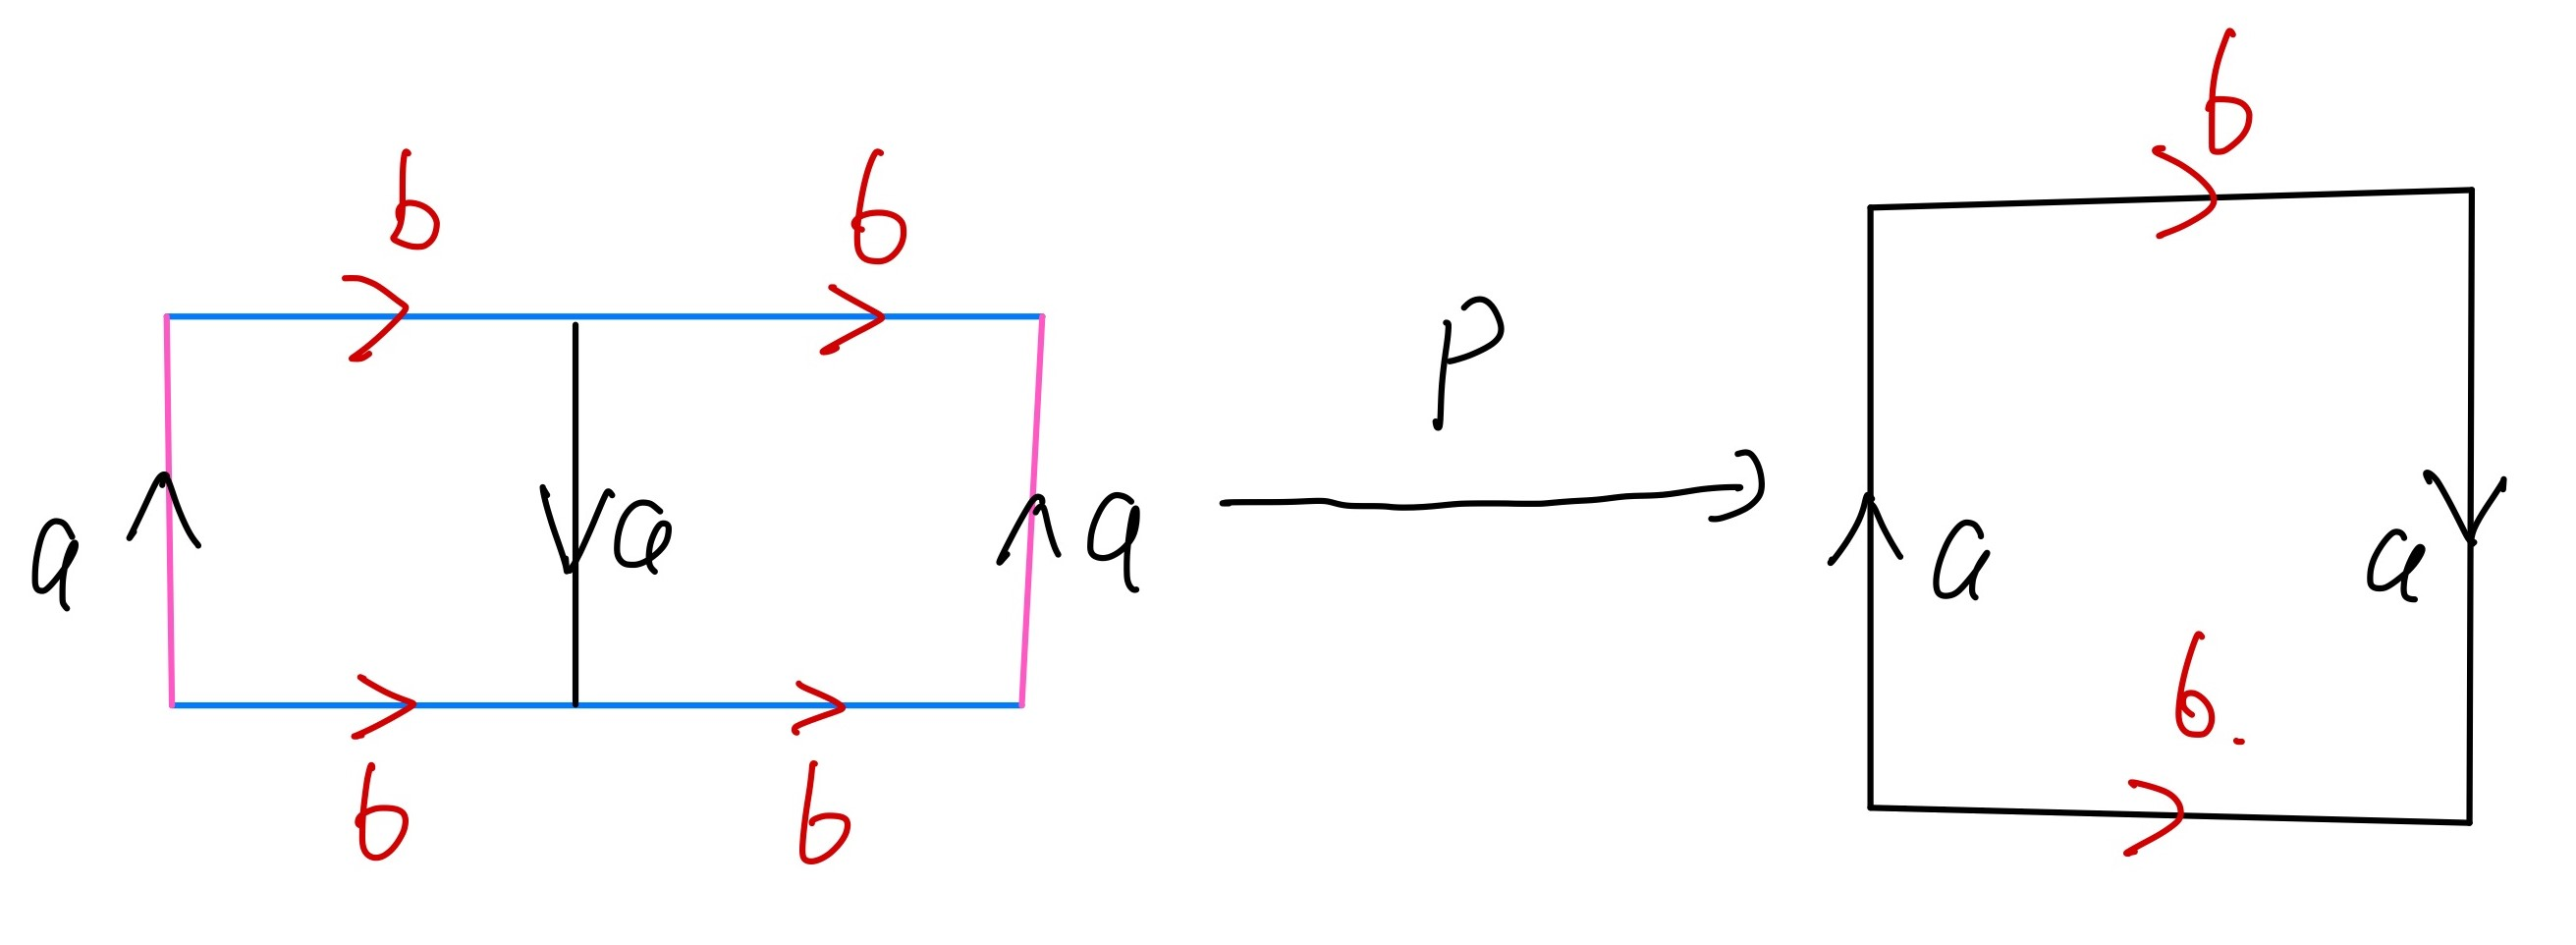
\includegraphics[scale=0.1]{Pictures/HW8-5-4.jpg}\]
The identification tells us the space is homeomorphic to the torus. 
\item Consider the last Cayley Graph. From a similar argument as above.
\[\mathbb{R}^2/\la a^2,b^2\ra=\left\{ (x,y)\in \mathbb{R}^2\mid 0\leq x,y\leq 2, (x,0)\sim (x,2), (0,y)\sim (2,y) \right\}.\]
Now we need to quotient out the subgroup generated by \(ab\). For a point \((x,y)\) on the integer grid, note that following the path \(b\) change the parity of the \(x\) coordinate, so we identify the point 
\((0,y)\) with \((1,1-y)\) if \(0\leq y\leq 1\), and identify \((0,y)\) with \((1,3-y)\). So the identification of the space gives a CW complex as follows 
\[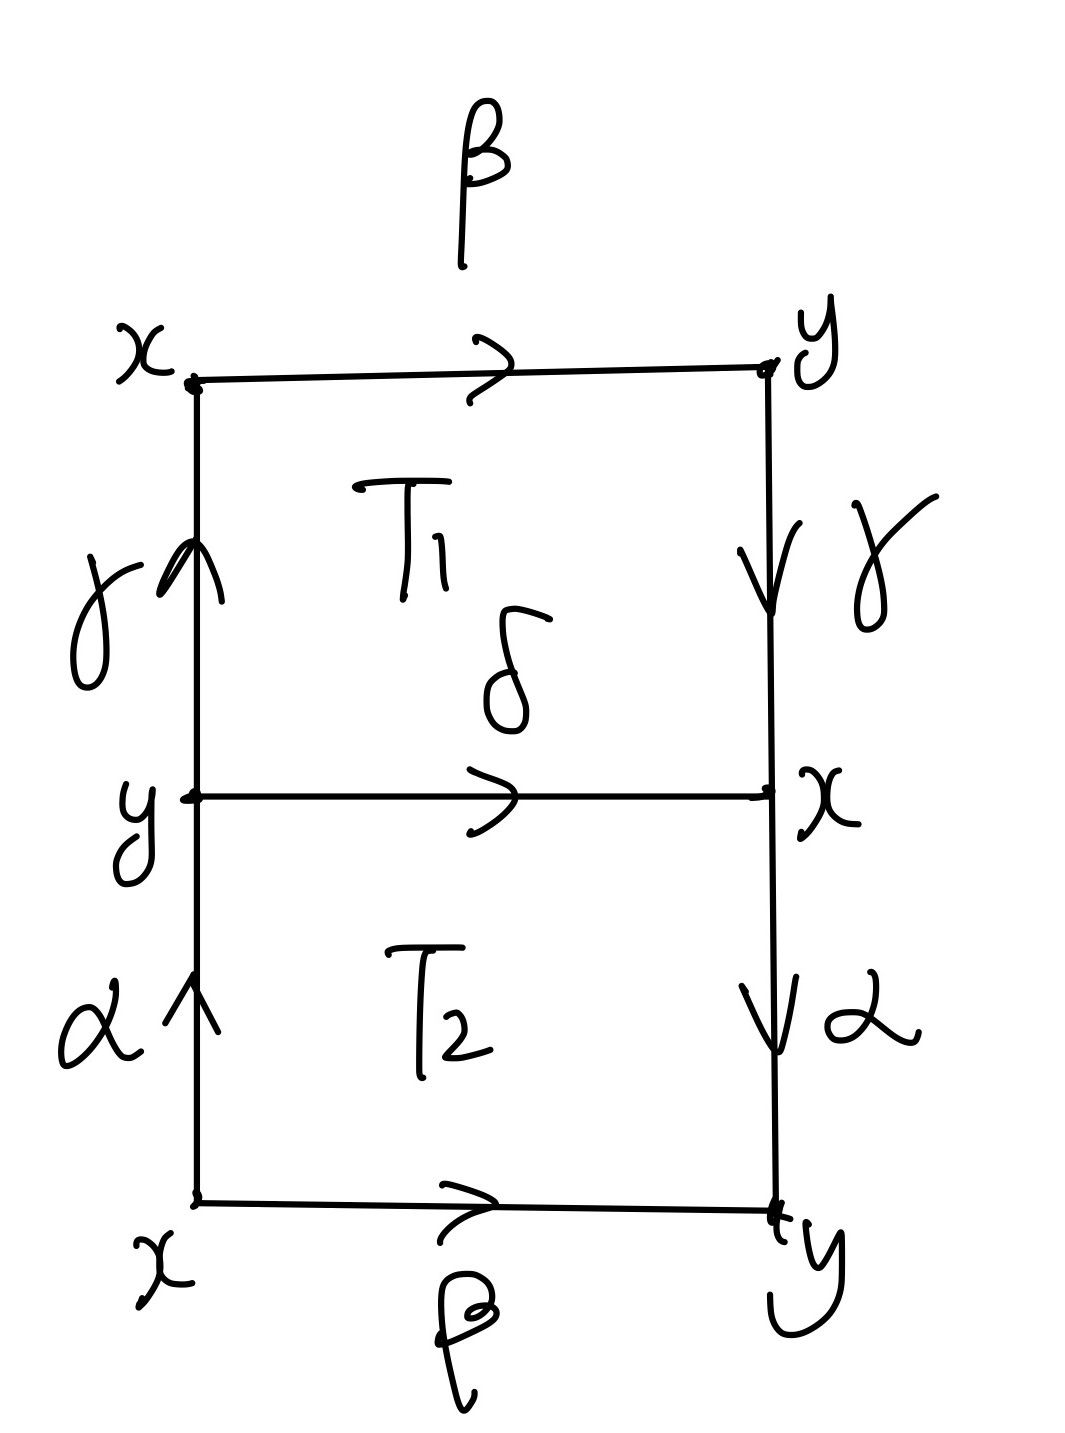
\includegraphics[scale=0.1]{Pictures/HW8-5-7.jpg}\]
Note that the Klein bottle has Euler characteristic \(0\), so the covering space must also have Euler characteristic 0, we know the only surface has Euler characteristic \(0\) is the Klein bottle or the torus. From the 
CW structure we can see that the second homology group \(H_2\) is trivial. So the covering is homeomorphic to the Klein bottle.
\end{enumerate} 
\item There are two connected Cayley Graphs of size 3:
\begin{figure}[h]
\begin{subfigure}{0.49\textwidth}
\centering
% https://q.uiver.app/#q=WzAsMyxbMCwwLCJzXzEiXSxbMiwwLCJzXzIiXSxbMSwyLCJzXzMiXSxbMCwxLCJiIiwwLHsiY29sb3VyIjpbMCw2MCw2MF19LFswLDYwLDYwLDFdXSxbMSwyLCJiIiwwLHsiY29sb3VyIjpbMCw2MCw2MF19LFswLDYwLDYwLDFdXSxbMiwwLCJiIiwwLHsiY29sb3VyIjpbMCw2MCw2MF19LFswLDYwLDYwLDFdXSxbMCwwLCJhIiwwLHsiYW5nbGUiOi00NX1dLFsxLDEsImEiLDAseyJhbmdsZSI6NDV9XSxbMiwyLCJhIiwwLHsiYW5nbGUiOi0xODB9XV0=
\begin{tikzcd}
	{s_1} && {s_2} \\
	\\
	& {s_3}
	\arrow["a", from=1-1, to=1-1, loop, in=100, out=170, distance=10mm]
	\arrow["b", color={rgb,255:red,214;green,92;blue,92}, from=1-1, to=1-3]
	\arrow["a", from=1-3, to=1-3, loop, in=10, out=80, distance=10mm]
	\arrow["b", color={rgb,255:red,214;green,92;blue,92}, from=1-3, to=3-2]
	\arrow["b", color={rgb,255:red,214;green,92;blue,92}, from=3-2, to=1-1]
	\arrow["a", from=3-2, to=3-2, loop, in=235, out=305, distance=10mm]
\end{tikzcd}
\caption{}
\end{subfigure}
\begin{subfigure}{0.49\textwidth}
\centering
% https://q.uiver.app/#q=WzAsMyxbMCwwLCJzXzEiXSxbMiwwLCJzXzIiXSxbMSwyLCJzXzMiXSxbMCwxLCJhIl0sWzEsMiwiYSJdLFsyLDAsImEiXSxbMSwyLCJiIiwyLHsiY3VydmUiOjIsImNvbG91ciI6WzAsNjAsNjBdfSxbMCw2MCw2MCwxXV0sWzIsMSwiYiIsMix7ImN1cnZlIjoyLCJjb2xvdXIiOlswLDYwLDYwXX0sWzAsNjAsNjAsMV1dLFswLDAsImIiLDIseyJhbmdsZSI6LTQ1LCJjb2xvdXIiOlswLDYwLDYwXX0sWzAsNjAsNjAsMV1dXQ==
\begin{tikzcd}
	{s_1} && {s_2} \\
	\\
	& {s_3}
	\arrow["b"', color={rgb,255:red,214;green,92;blue,92}, from=1-1, to=1-1, loop, in=100, out=170, distance=10mm]
	\arrow["a", from=1-1, to=1-3]
	\arrow["a", from=1-3, to=3-2]
	\arrow["b"', color={rgb,255:red,214;green,92;blue,92}, curve={height=12pt}, from=1-3, to=3-2]
	\arrow["a", from=3-2, to=1-1]
	\arrow["b"', color={rgb,255:red,214;green,92;blue,92}, curve={height=12pt}, from=3-2, to=1-3]
\end{tikzcd}
\caption{}
\end{subfigure}
\end{figure}

The stabilizers can be written as 
\begin{align*}
	(a)&\ \ \Stab(s_1)=\la a,b^3\ra,\\ 
	(b)&\ \ \Stab(s_1)=\la b, a^3\ra.
\end{align*}
Let us find the covering space corresponding to the Cayley Graph \((a)\) and \((b)\).
\begin{enumerate}[(a)]
\item The covering space is shown as below: 
\[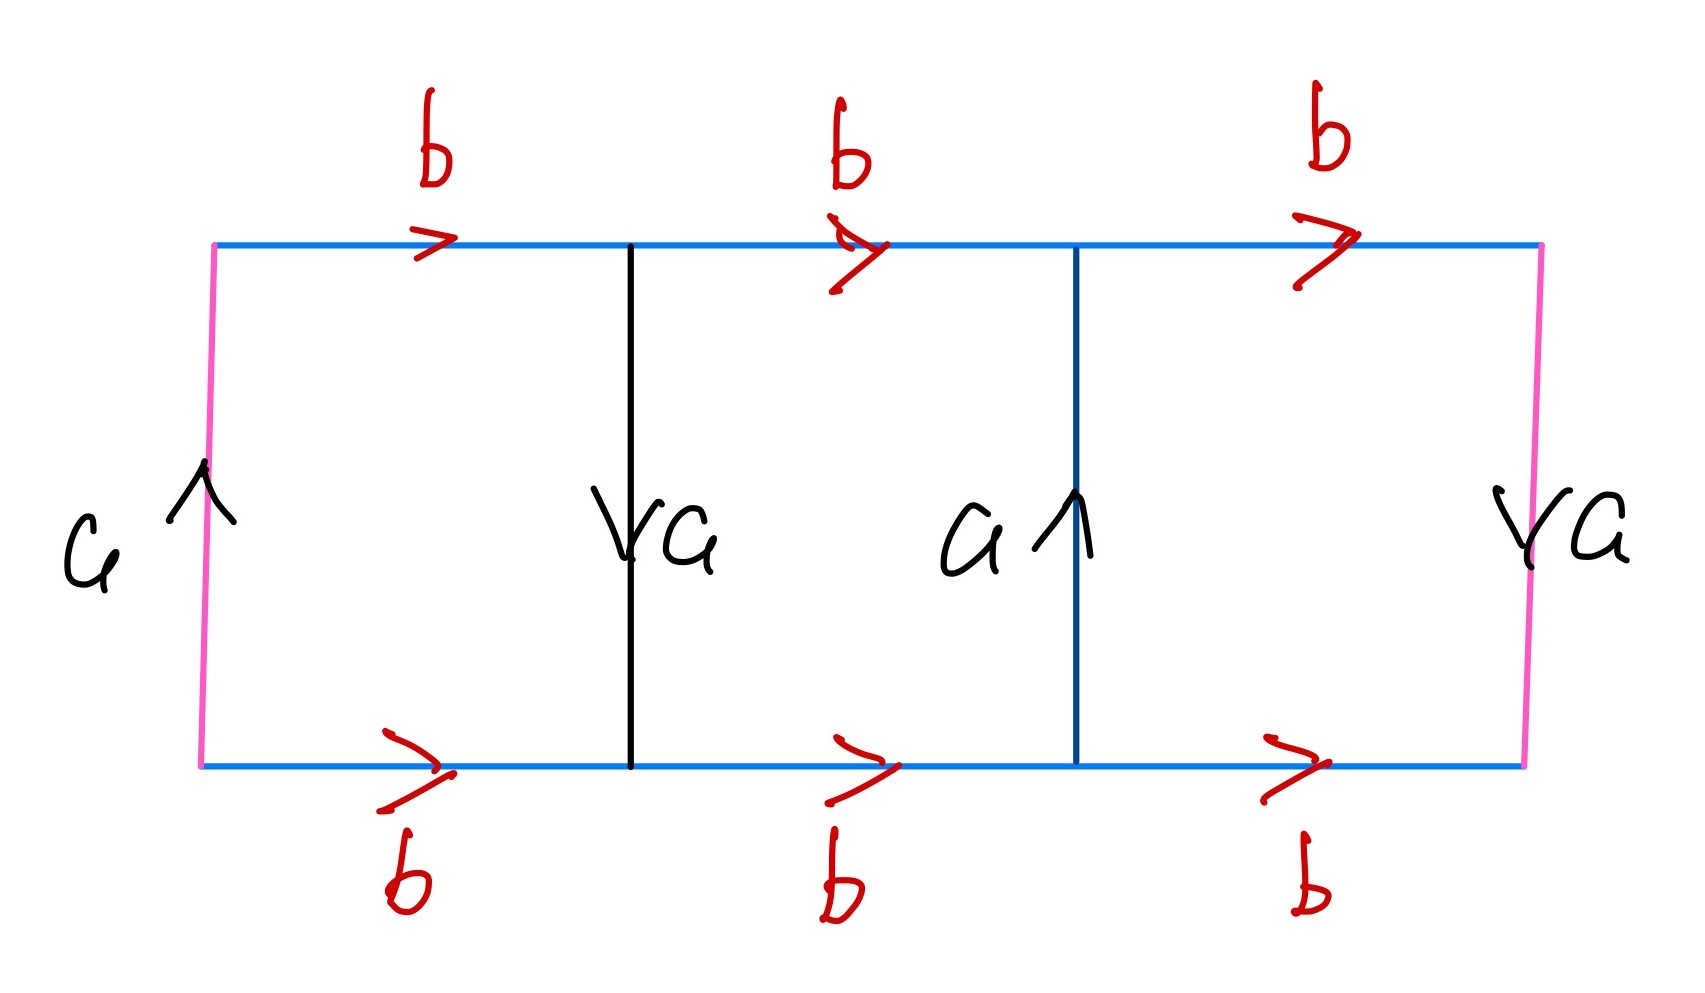
\includegraphics[scale=0.1]{Pictures/HW8-5-5.jpg}\]
From a similar argument we can see that 
\[\mathbb{R}^2/\la a,b^3\ra=\left\{ (x,y)\in \mathbb{R^2}\mid 0\leq x\leq 3,0\leq y\leq 1, (x,0)\sim (x,1), (0,y)\sim (3,1-y) \right\}.\]
Note that \((0,y)\sim (1,1-y)\) because following the path \(b^3\) changes the parity of \(x\) coordiante (even \(\leftrightarrow \) odd), this changes the direction of path \(a\). 
The identification tells us this is homeomorphic to the Klein bottle.
\item The covering space is shown as below: 
\[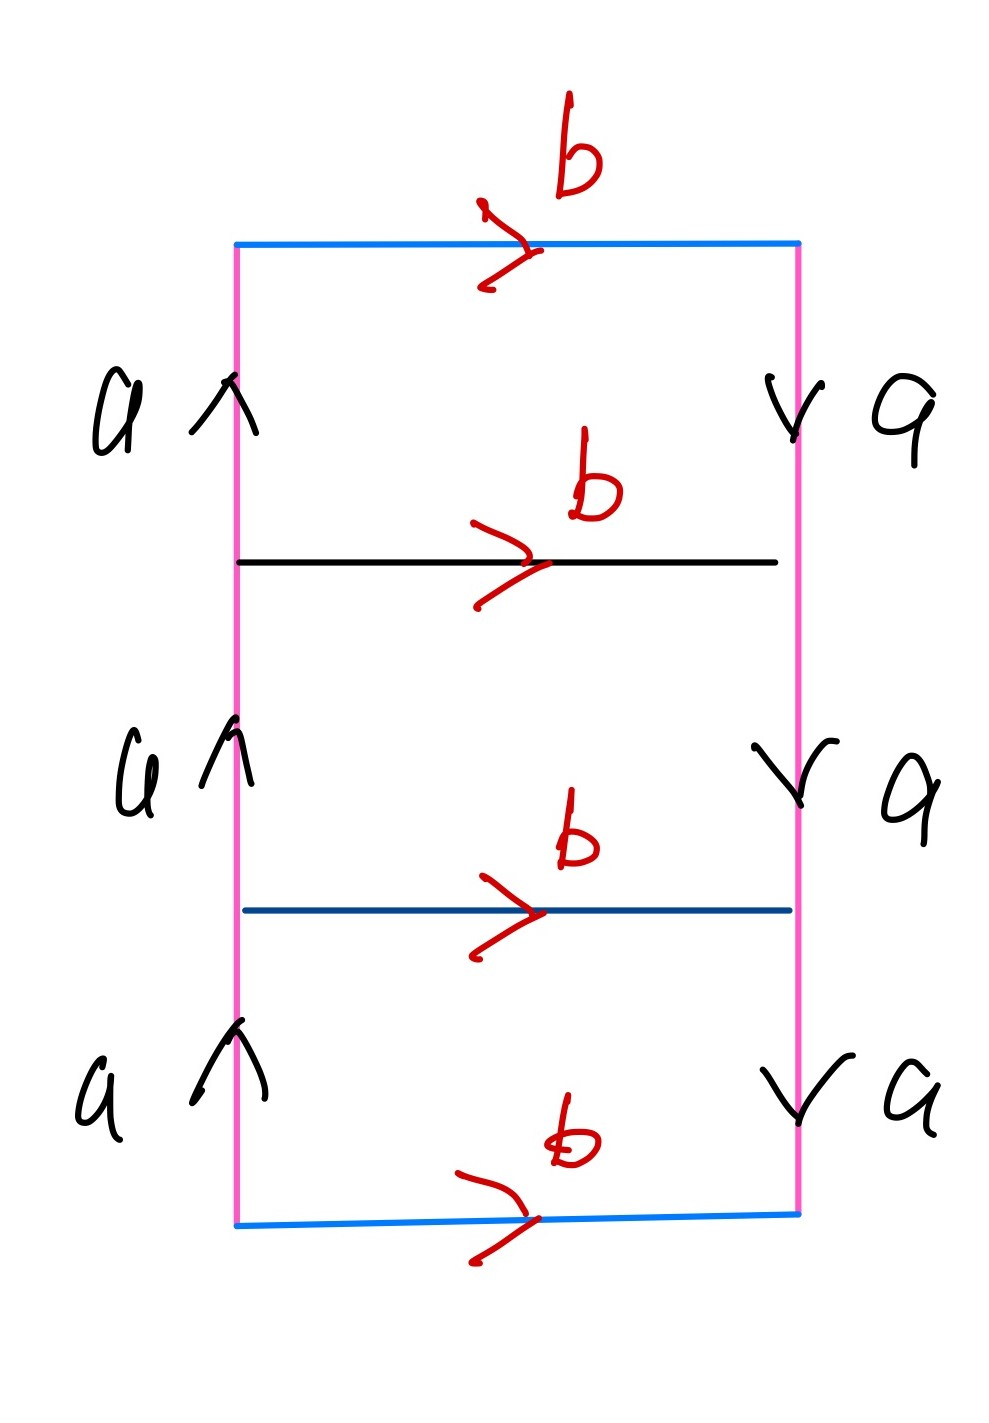
\includegraphics[scale=0.1]{Pictures/HW8-5-6.jpg}\] 
Similarly, we can see that 
\[\mathbb{R}^2/\la b,a^3\ra=\left\{ (x,y)\in \mathbb{R}^2\mid 0\leq x\leq 1,0\leq y\leq 3, (x,0)\sim (x,3),(0,y)\sim (1,3-y) \right\}.\]
The identification tells us this is homeomorphic to the Klein bottle.
\end{enumerate}
\end{enumerate}
\end{solution}


\end{document}